\documentclass[english,phd]{diploma}

% Packages
\usepackage[autostyle=true]{csquotes} % enhanced support for quotation marks, support for biblatex package
\usepackage[backend=biber, style=iso-numeric, alldates=iso, maxbibnames=3]{biblatex}
\usepackage{dcolumn} % numeric column type
\usepackage{subfig} % subtables and subfigures
\usepackage[cpp]{diplomalst}
\usepackage{hyperref}
\usepackage{todonotes}
\usepackage{tikz}
\usetikzlibrary{graphs}
\usetikzlibrary{positioning}
\usetikzlibrary{arrows.meta}
\usetikzlibrary{math}

% Fix arrow tips
\tikzset{tips=proper}

% Commands
\newcommand{\comment}[1]{}

% Tools
\newcommand{\estee}{\emph{Estee}}
\newcommand{\rsds}{\emph{RSDS}}
\newcommand{\hyperqueue}{\emph{HyperQueue}}
\newcommand{\dask}{\emph{Dask}}
\newcommand{\ray}{\emph{Ray}}
\newcommand{\snakemake}{\emph{SnakeMake}}

% TikZ styles
\tikzset{%
    task/.style={circle, draw},
    data/.style={rectangle, draw, rounded corners},
    arrow/.style={draw, thick, {->}}
}

% Metadata
\ThesisAuthor{Ing. Jakub Beránek}

\ThesisSupervisor{Ing. Jan Martinovič, Ph.D.}

\CzechThesisTitle{Ergonomie a efektivita workflow na HPC klastrech}
\EnglishThesisTitle{Ergonomics and efficiency of workflows on HPC clusters}

\SubmissionYear{2023}

\Acknowledgement{I would like to thank all those who helped me with the work, because without
them this work would not have happened.}

\CzechAbstract{TODO}
\CzechKeywords{distribuované výpočty, výpočetní grafy, vysokovýkonnostní počítání}

\EnglishAbstract{TODO}
\EnglishKeywords{distributed computing, task workflows, hpc}

\addbibresource{references.bib}
\addbibresource{publications.bib}

\begin{document}
\MakeTitlePages

\listoffigures
\clearpage

\listoftables
\clearpage

\chapter{Introduction}
\label{ch:Introduction}
High Performance Computing (HPC) infrastructures are crucial for the advancement of scientific
research, as they offer unparalleled computational power that can be leveraged to perform the most
complex scientific experiments. The performance offered by HPC clusters is crucial (among other
use-cases) in various scientific areas, such as weather forecasting~\cite{wrf},
computational fluid dynamics~\cite{cfd}, bioinformatics~\cite{bioinformatics} or deep
learning~\cite{hpcdl}.

Over the last several decades, the performance of HPC clusters (and also consumer computing
devices) has been steadily increasing, effectively doubling every few years, in line with the
implications of Moore's Law and Dennard scaling\todo{cite?}. However, it also became more
difficult for HPC users to tap into that performance increase. Thirty years ago, it was possible to
buy a new (super)computer every two years and get essentially doubled performance for free, without
having to modify existing programs. This phenomenon has started to diminish by the end of the last
century, as chip designers became limited by the memory wall~\cite{memorywall} and especially
the power wall~\cite{powerwall}.

To keep up with the exponential performance increases, processors had to become more complex,
gaining many buffers and caches, multiple cores, simultaneous multithreading, out-of-order
execution and a plethora of other techniques to make them run faster. The existence of multiple
cores and sockets and the need for ever-increasing memory sizes has also made the memory system
more complex, with NUMA (Non-Uniform Memory Access) memories becoming commonplace in HPC\@. To gain
even more performance, HPC clusters started massively adopting various accelerators, like the Intel
Xeon Phi~\cite{xeonphi} manycore coprocessor or general-purpose Graphics processing units
(GPUs) from NVIDIA or AMD, which became the backbone of a majority of current
supercomputers\todo{cite?}. Some clusters have also adapted more unconventional
accelerators, like reconfigurable hardware (e.g.\ Field-programmable gate arrays) or Artificial
Intelligence (AI) accelerators (e.g.\ Tensor processing units). This trend gave rise to
heterogeneous clusters, that offer various types of hardware that are designed for specific
workloads.

The increasing complexity and heterogeneity of HPC hardware has caused the ``HPC software stack''
and the corresponding programming models to also become more complex. Making full use of the
available performance is far from trivial. Computing nodes consisting of hundreds of cores make it
quite challenging to write programs that can scale to such high core counts. Main memory being
split into multiple physical locations with various access latencies (NUMA) and complex memory
hierarchies require specialized programming techniques to achieve optimal performance. And using
the ever-present accelerators, for example GPUs, might require adopting a completely new
programming model.

Historically, optimized HPC software was usually written using system or scientifically focused
programming languages (e.g.~\texttt{C}, \texttt{C++} or
\texttt{Fortran}) and specialized libraries for parallelizing and distributing computation
(such as OpenMP, CUDA or MPI)~\cite{mpistudy}. While these rather low-level technologies are
able to provide the best possible performance, it can be quite challenging and slow to develop (and
maintain) applications that use them. It is unreasonable to expect that most domain scientists that
write software which runs on HPC resources (who are often not primarily software developers) will
be able to use all these technologies in an efficient manner without making the development process
slow and cumbersome. This task should be left to specialized performance engineers, enabling the
scientists to focus on the problem domain~\cite{dace}.

With the advent of more powerful hardware and more advanced software, the computations performed on
HPC systems are also becoming more demanding, both in terms of the required computational power,
but also software design and architecture. Areas such as weather prediction, machine learning model
training or big data analysis require executing thousands or even millions of simulations and
experiments. They also typically require a lot of prototyping during development. These experiments
can be quite complex, consisting of multiple dependent steps, such as data ingestion,
preprocessing, computation, postprocessing, visualisation, etc. It is thus imperative for
scientists to have a quick way of prototyping these applications, otherwise their development
process would be quite slow.

The growing complexity of HPC hardware, software and use-cases gave rise to the popularity of
task-based programming models and paradigms. The term \emph{task-based programming} is used for a lot of
related technologies and programming models, ranging from fine-grained tasks that execute a single
function or just a handful of instructions~\cite{starpu,openmp} to coarse-grained task workflows
that execute binaries which can run for hours or even days~\cite{dask, snakemake, nextflow}. This
thesis primarily focuses on the latter type of task graphs, which represent very general
computations (either functions or binaries) with various levels of granularity,
that are intended to be distributed among multiple nodes of a distributed cluster.

The task graph programming model allows users to focus on the problem domain and quickly prototype,
while still being able to describe complicated computations with a large amount of individual steps
and to efficiently utilize the available computational resources. Using a task-based approach, a
computational workflow is described using a set of atomic computational blocks
(\emph{tasks}) that are composed together in a \emph{task graph} which captures the
dependencies between the individual tasks. Task graphs abstract away most of the complexity of
network communication and parallelization, and they are general enough to describe a large set of
programs in a practical and simple way. At the same time, they remain amenable to compiler-driven
optimization and parallelization, which helps to bring the performance of programs described by a
task graph close to manually parallelized and distributed programs, at a fraction of the
development cost for the application developer. They are also quite portable. The task graph
programming model does not make many assumptions about the target platform, therefore the same task
graph can be executed on various systems and clusters, provided there is an execution runtime
implemented for that cluster.

Combined with the fact that task-based tools often allow users to write their program in very
high-level languages, such as Python, or various domain-specific languages (DSLs), it makes them an
ideal tool for rapid scientific prototyping\todo{cite}.

Task graphs are already commonly being used and deployed on various distributed
systems\todo{cite}, yet there are certain challenges that limit their development
productivity and scalability when deployed specifically on HPC systems. These challengs stem from
various factors, such as the interaction of task-graph runtimes with HPC job managers,
heterogeneity and complexity of HPC cluster hardware, or simply from the sheer computational scale
of HPC systems. Removing or alleviating some of those challenges could lower the barrier of entry,
make task graph execution better suited for various HPC use-cases and turn it into an actual
first-class citizen in the world of HPC.

This thesis aims to improve the execution of task graphs on HPC systems in two main areas,
developer ergonomics and efficient hardware utilization. The combination of a simple and ergonomic
programming model with efficient execution on a distributed cluster is the key strength of task
graphs, yet they have various shortcomings when applied in HPC environments. The objective of this
thesis is to identify these bottlenecks and reduce their negative effect (or remove them
altogother). This thesis aims to achieve this objective via the following contributions:
\begin{itemize}
	\item Analysis of the performance and usability of contemporary task runtimes and the challenges that
	      they face in HPC environments.
	\item Analysis of the scheduling quality of task schedulers based on various conditions and the
	      introduction of \estee{}, an environment for experimentation with different scheduling
	      algorithms.
	\item \rsds{}, a distributed task runtime compatible with an existing task framework
	      (\dask{}), which is optimized for HPC use-cases.
	\item Design of an approach to reconciliate task graphs with HPC job managers, to reduce the barrier of
	      task graph execution on HPC clusters.
	\item \hyperqueue{}, an integrated, HPC focused tool for executing task graphs on HPC systems
	      in an ergonomic and efficient manner.
\end{itemize}

The thesis is structured as follows. Chapter~\ref{ch:taskgraphs} introduces the task graph
programming model. Chapter~\ref{ch:challenges} then discusses various challengs of executing
task graphs on HPC systems. It is followed by Chapter~\ref{ch:sota}, which contains a
taxonomy of selected task runtimes and analyses their behavior in HPC environments. TODO TODO TODO.
Finally, Chapter~\ref{ch:conclusion} summarizes the thesis and outlines future work.


\chapter{Task-based programming model}
\label{ch:taskgraphs}
In order to discuss task-based programming, it is useful to provide a vocabulary of terms related
to it. This vocabulary necessarily has to be relatively general, in order to be applicable to a
wide range of systems; even though the previous chapter has specified a precise subset of
task-based programming models that will be examined and analyzed in this thesis, there is still a
large number of tools and systems that belong to this area of interest, each with their own
distinct concepts and semantic rules. Therefore, it is infeasible to provide a single unifying and
complete task theory that would encompass details of all these tools and programming models.

This chapter defines a set of concepts related to tasks, with a particular focus on properties that
are important for task graph execution in \gls{hpc} environments, which will be
further described in~\Autoref{ch:sota}. The definitions described in this chapter are
specifically adapted to the needs and terminology of this thesis, as is usual for other research
works. They form the lowest common denominator that can be applied to the specific task execution
tools and their programming models discussed throughout this thesis. The presented terms are
similar to definitions that can be found in existing works~\cite{task_scheduling,hagras2003static,wang2018list}. However, they
differ in several aspects. In particular, we do not assume that task execution times nor output
data sizes are known in advance, and we provide a very general definition of task resource
requirements, which can be used to model complex resource management of heterogeneous clusters.

\section{Task graphs}
\label{sec:task-graphs}
A computational workflow in the task-based programming model is represented with a
\gls{dag} that we will label as a \emph{task graph}. From a high-level
perspective, it describes which individual computational steps should be performed, what are the
constraints for where and in which order they should be computed and how should data be transferred
between the individual steps of the workflow.

There are many variations of task graphs, based on the computational properties that they are able
to describe. In the most basic form, task graph vertices represent computations to be performed,
and the arcs (edges) represent dependencies between the computations, which enforce an order in
which they should be executed. However, numerous other concepts can also be encoded in a task
graph. For example, in addition to dependencies, the arcs could represent abstract communication
channels, through which the outputs of one computation are transferred to become the inputs of
another computation that depends on it. As another example, there could be a special type of arc
which specifies that the outputs of a computation will be streamed to a follow-up computation,
instead of being transferred in bulk only after the previous computation has finished.

As was already noted, the exact semantics of vertices and arcs of task graphs depend heavily on the
specifics of tools that implement them, and thus it is not possible to provide a single definition
that would fit all variants used ``in the wild''. To provide a baseline definition, we will
formally define a task graph that can capture dependencies between tasks, the notion of
transferring data outputs between tasks, and where tasks can specify resources needed for their
execution.

\newcommand{\alltaskpairs}{\forall t_1\in{}T, \forall t_2\in{}T}

A task graph is a tuple $(T, O, E, \setresourcekinds, \fntaskres)$, where:
\begin{itemize}[itemsep=0pt]
	\item $T$ is a set of \emph{tasks}.
	\item $O$ is a set of \emph{data objects}.
	\item $E \subseteq ((T\times{}O) \cup (O\times{}T))$ is a set of arcs.
	\item $\setresourcekinds$ is a set of \emph{resource kinds}. Each resource kind describes some resource
	      (e.g. \gls{cpu} cores or \glspl{gpu})
	      that is required to execute a specific task.
	\item[\makedef{def:task_resreq}] $\fntaskres$ is a function that defines the
		\emph{resource requirement} of a task for a specific resource kind: \\
		\resourcerequirement{\fntaskres}{N} \\
		A resource requirement specifies what amount of the given resource kind is required to be present
		at a computational provider so that the task can be executed. If $\fntaskres(t, r) = 0$, then task
		$t$ does not require resource $r$ for its execution.
\end{itemize}

$(T \cup O, E)$ forms a finite directed acyclic graph (a graph without cycles). The graph is
structured in a way so that for every data object, there is exactly one task that produces it: \\
$\forall o \in O: |E \cap (T \times \{o\})| = 1$

\vspace{2mm}Below we will define several terms that will be useful for describing task
graphs and their properties:
\begin{itemize}
	\item If there is an arc from a task to a data object ($(t,o) \in (T\times{}O)$), then we call
	      $t$ the \emph{producer} of $o$ and
	      $o$ the \emph{output} of $t$.
	\item If there is an arc from a data object to a task ($(o,t) \in (O\times{}T)$), then we call
	      $t$ the \emph{consumer} of $o$ and
	      $o$ the \emph{input} of $t$.

	\item Let us introduce a binary relation $D_r$: \\ $D_r: T \times T = \{(t_1, t_2) \mid (t_1, t_2)\in{}(T\times{}T)\land t_1 \neq t_2 \land
		      \exists{}o\in{}O\colon (t_1, o)\in{}E
		      \land (o, t_2)\in{}E\}$ \\ When
	      $(t_1, t_2) \in D_r$, we say that $t_2$ \emph{directly depends} on
	      $t_1$. We can also state that $t_2$ consumes the output produced
	      by $t_1$.

	\item Let us introduce a binary relation $D$: \\ $D: T \times T = \{(t_1, t_2) \mid \exists{}n (t_1, t_2, \ldots, t_n)\colon \forall i
		      \in \{1,2,\ldots,n - 1\}\colon (t_i, t_{i+1}) \in{} D_r\}$ \\ When
	      $(t_1, t_2) \in D$, we say that $t_2$ \emph{depends} on
	      $t_1$ and that $t_1$ is a \emph{dependency} of
	      $t_2$.

	\item We label tasks without any dependencies \emph{source tasks}: \\ $S = \{ t \mid t\in{}T \land
		      \forall{}t_d\in{}T\colon (t_d, t)\notin D\}$ \\ It is
	      a simple observation that unless the task graph is empty ($(T\cup{}O) = \emptyset$), there is always
	      at least one source task in the graph, because the graph is acyclic.
\end{itemize}

% \footnote{This representation will be used in all following task graph diagrams.}

An example of a simple task graph is shown in~\Autoref{fig:task-graph-example}. Tasks are represented as
circles, data objects as (rounded) rectangles and arcs as arrows. The task $t_0$
generates two data objects, which are then used as inputs for four additional tasks. The outputs of
these four tasks are then aggregated by a final task $t_5$. This can correspond
e.g.\ to a workflow where $t_0$ generates some data, $t_{1-4}$
performs a calculation on that data and $t_5$ then performs a final
post-processing step and stores the results to disk.

\begin{figure}[h]
	\centering
	\resizebox{!}{35mm}{
	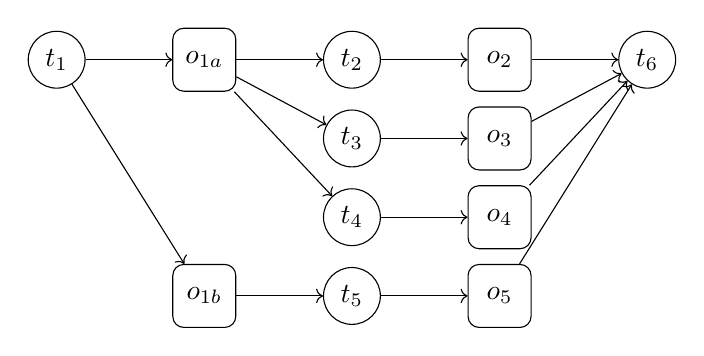
\begin{tikzpicture}
			\tikzset{%
				data/.style={rectangle, draw, rounded corners, minimum size=8mm},
			}
            \graph[
                grow right sep=11mm,
            ] {
                "$t_1$"[task] -> {
                    "$o_{1a}$"[data] -> {
                        "$t_2$"[task] -> "$o_{2}$"[data],
                        "$t_3$"[task] -> "$o_{3}$"[data],
                        "$t_4$"[task] -> "$o_{4}$"[data]
                    },
                    "$o_{1b}$"[data] -> {
                        "$t_5$"[task] -> "$o_{5}$"[data]
                    }
                } -> "$t_6$"[task]
            };
        \end{tikzpicture}
	}
	\caption{Simple task graph with six tasks and six data objects}
	\label{fig:task-graph-example}
\end{figure}

Note that the presented definition of a task graph does not describe its semantics -- how will the
graph be created and executed and what will be the interactions between tasks and data objects.
This depends on the specific tool or framework that will execute the task graph. As an example, the
dependence of task $t_2$ on task $t_1$ could define the following
invariant: $t_2$ cannot start to execute until $t_1$ has finished
executing and the data objects produced by $t_1$ have been transferred to the
computational node that will execute $t_2$. A formal definition of a basic set of
execution and scheduling semantics will be provided in~\Autoref{sec:task-scheduling}.

A \emph{task} is a serializable description of a computation that can be executed
repeatedly. The serializability property is crucial, as it allow us to treat computation as data.
That is a powerful concept, because it allows tasks to be sent between different nodes in a cluster
or stored to disk and to be transparently recomputed an arbitrary number of times. Enabling the
recomputation of tasks is useful for achieving fault tolerance, as tasks might need to be
recomputed later if some failure occurs during their execution.

In practice, a single task will typically represent either the invocation a function (an executable
block of code) or the execution of a whole program. Multiple tasks in a task graph can refer to the
same function or program, since each such task can have different inputs. In fact, this is a common
case, as task graphs are often used to parametrize a small set of functions or programs with many
different input parameters.

Even though the inputs and outputs of tasks were defined as sets in the formal definition, in
practice they are usually stored using either ordered sequences or a mapping that associates a name
with each input or output, because it is important to maintain a specific ordering of both inputs
and outputs. For functions, the inputs are passed as arguments, and the output is derived from its
return value (which can potentially form a sequence of values). Therefore, we have to be able to
associate each task input to a specific argument index. The same holds for tasks that execute
programs. In this case, inputs can be mapped to command-line arguments and the content of the
\texttt{standard input stream}, and the output can be e.g.\ the content of the \texttt{standard output stream}
generated by the executed program.

Each task can define its \emph{resource requirements}, a set of constraints for the worker(s) that are
able to execute that task. As an example, a task that performs training of a machine-learning model
might require a \gls{gpu} to be present on the worker where the task will be executed.
Other resources might include e.g.\ a specific number of \gls{cpu} cores or a minimum
amount of \gls{ram} or necessary to execute a given task.

A \emph{data object} represents a dynamically computed result of a task; it is not known at the
time of the task graph creation. Typically, it is a serialized blob of data that is eventually
transferred from the node where its producer was computed to the node where its consumer should be
executed. If a task programming model does not encode direct data transfers between tasks, then
data objects simply serve as ``empty'' markers of dependencies, and they do not hold any actual
data. In that case, we could even remove them from the task graph completely, and represent task
dependencies directly with arcs between tasks.

It is important to note that not all data used by tasks has to be encoded as a data object in the
task graph. As an example, tasks that represent function invocations are usually created by the
execution of some program (e.g.\ a Python script). A task graph defined in this way is usually
constructed with a specific set of input data for its \emph{source tasks}. This data can be
embedded directly within the definition of the function itself; in that case it is not represented
as an explicit data object. In other words, a task might represent a serializable description of a
computation along with its input data. That is why in the presented formal definition,
\emph{source tasks} do not have any explicit \emph{inputs}, as it is expected that
input data is embedded directly within them.

Additionally, when a task is executed, it can also read and modify the state of the environment in
which it is being executed, in a way that is observable by other tasks. For example, a function can
read or modify the value of a global variable, while a program can read an environment variable or
create a file on a disk, without it being specified as a task output. Such actions, which we will
label as \emph{side effects}, are also typically not encoded within the task graph. Tasks should
ideally contain as few side effects as possible, because they can make task execution
non-deterministic, causing them to produce different outputs when executed multiple times, which is
typically undesirable.

In general, the most important goal of the task graph is to encode high-level structure of the
computation (such as dependencies between tasks), which enables a task execution tool to
automatically execute the task graph in a parallel fashion. However, many details about the
computation itself are specified outside the task graph itself.

\section{Task execution}
Task graphs merely describe some computation; therefore, they have to be executed in order to
actually produce some outputs and results. This is the responsibility of a \emph{task runtime},
a tool that analyzes task graphs and executes them in some \emph{computational environment}, e.g.\ a personal
computer or a distributed cluster. Such an environment contains a set of computational providers
that are able to execute tasks. We will label these providers as \emph{workers}. A worker
can execute a task by invoking the computation assigned to it (typically by calling a function or
executing a program), and passing it the inputs of the task. Usually a task can only be executed
once all of its inputs are ready, which means that the dependencies of the task have been computed,
and their outputs have been transferred to the computational node of the worker. However, this
depends on the semantics of each task runtime.

We can formally define a \emph{computational environment} as a tuple $(W, \setresourcekinds, \fnworkerres)$, where:
\begin{itemize}[itemsep=0pt]
	\item $W$ is a set of workers.
	\item $\setresourcekinds$ is a set of \emph{resource kinds}. Each resource kind describes some
	      resource (e.g. \gls{cpu} cores or \glspl{gpu}) that can be provided a
	      worker.
	\item[\makedef{def:worker_resources}] $\fnworkerres$ is a function which defines how many resources are
		provided by a worker for a specific resource kind: \\ $\fnworkerres\colon W \times \setresourcekinds \rightarrow
			\mathbb{N}_{\geq{}0}$
\end{itemize}

There are many existing task runtimes with varying architectures, features and trade-offs, which
affect factors like performance, fault tolerance or expressivity of the supported variant of the
task-based programming model. Several task runtimes will be discussed throughout this thesis. In
the rest of this section, we will consider a case typical for \gls{hpc} environments;
a distributed task runtime with a central manager that communicates with a set of workers running
on remote nodes that communicate together via a network.

In general, a task runtime oversees all aspects of task graph execution. Its two main
responsibilities can be divided into managing communication with the workers, and handling the
scheduling and execution of tasks.

Worker management involves handling the lifetime of workers (connection and disconnection from the
cluster), facilitating data transfers between them or providing resiliency in case of worker
failures. A single worker is typically a program running on a computational node, which is
connected to the runtime manager. It receives commands from it, executes tasks and sends
information about task execution statuses back to the manager. Each worker typically manages some
hardware resources that are available for tasks during their execution. Hardware resources can be
assigned to workers in various ways. There can be a single worker per the whole computational node,
or there could be multiple workers per node, each managing a subset of the available resources
(e.g.\ a single worker per \gls{cpu} core).

The second main aspect that has to be handled by the runtime is the management of tasks. It has to
keep track of which tasks have already been computed, which tasks are currently being executed on
some worker(s) or which tasks are ready to be executed next, because their dependencies have
already been computed. Two important responsibilities in this area are fault tolerance and
scheduling.

In the context of task graph execution, we will define \emph{fault tolerance} as the ability to
gracefully handle task execution failures, and provide ways of retrying failed computations. When
the execution of a task fails with some error condition (e.g.\ because a worker executing the task
crashes), a fault-tolerant task runtime will be able to transparently restart it by launching a new
execution of that task. We will use the term \emph{task instance} for a specific execution of a
task. Runtimes might impose some limits on retrying failed tasks, e.g.\ by attempting to execute up
to a fixed number of task instances for each task before giving up, to avoid endless failure loops.

The fact that it is even possible to execute a task multiple times is one of the main advantages of
the task-based programming model, where tasks declaratively describe a self-contained computation
that can be re-executed arbitrarily many times. This crucial property of tasks makes fault-tolerant
execution of task graphs easier to achieve than in other programming models, where individual
computations are not self-contained and serializable.

\section{Task scheduling}
\label{sec:task-scheduling}
One of the most important responsibilities of a task runtime is \emph{task scheduling}. It is the
act of deciding in which order and on which specific worker(s) should each task execute, in a way
that optimizes some key metric. We will use the term \emph{scheduler} for a component of the
task runtime that is responsible for assigning tasks to workers by creating
\emph{schedules}. A schedule is a mapping that assigns tasks to specific workers that should
execute them, and also assigns an order in which the tasks should be executed. It can be
\emph{static}, in which case it is produced just once before the task graph begins
executing, or \emph{dynamic}, where the scheduler generates the assignments on-the-fly,
based on the current utilization of workers and the observed durations of tasks that have already
been executed. Some schedulers also retroactively modify already produced schedules in reaction to
dynamic situations that occur during task graph execution (e.g.\ if a new worker connects to the
cluster, or if some worker is starving).

We will split the formal definition of a \emph{schedule} into two parts, because the
schedule decides both the worker that executes a given task, and also the ordering in which tasks
are executed. As mentioned earlier, a schedule can be produced either before the task graph is
executed or during its execution. The following definitions are general and work for both
approaches.

We can define a \emph{schedule} as a pair $(\scheduleworker, \scheduleorder)$ applied to a task graph
$(T, O, E, \setresourcekinds, \fntaskres)$ and a computational environment $(W, \setresourcekinds, \fnworkerres)$ as follows:

\begin{itemize}[itemsep=0pt]
	\item A worker schedule $\scheduleworker$ is a function that assigns each task to a specific worker:
	      \\ $\scheduleworker\colon T \rightarrow W$
	\item An ordering schedule $\scheduleorder$ is a function that assigns a unique number to each
	      task, to define an (approximate) ordering in which tasks should be executed: \\
	      $\scheduleorder\colon T \rightarrow \mathbb{O}, \mathbb{O} =
		      \{1,\ldots,|T|\},
		      \alltaskpairs\colon \scheduleorder(t_1) = \scheduleorder(t_2) \Rightarrow t_1 = t_2$
\end{itemize}

This definition supports only single-node tasks, i.e.\ tasks that are always executed on exactly a
single node. It could be generalized for other use-cases that have a more complex programming
model. For example, we could add support for multi-node tasks by generalizing the worker schedule
to be a mapping of tasks to a non-empty set of workers: \\ $\scheduleworker\colon T \rightarrow \powerset{W}, \forall
	t\in{}T\colon |\scheduleworker(t)| > 0$

Usually, we will want the produced schedules to have additional desirable properties, such as
respecting the dependencies and resource requirements of tasks in the task graph. Even though the
specifics of these properties differ in each task-based programming model, we can define a set of
baseline properties that are desirable in almost all situations. In order to do that, we will need
to consider a specific execution of a task graph that used a given schedule; we can then evaluate
whether that schedule satisfied these properties in the context of this execution.

Assume that we want to evaluate a specific schedule ($\scheduleworker$,
$\scheduleorder$) that was used to execute a task graph $(T, O, E, \setresourcekinds, \fntaskres)$ in a
computational environment $(W, \setresourcekinds, \fnworkerres)$ in some execution $X$. For
simplicity, we assume exactly one task instance executed for each task. In other words, tasks in
this execution did not fail and each task was fully executed. First, let us define several
auxiliary functions:

\newcommand{\timedomain}{\mathbb{R}_{\geq{}0}}

\begin{itemize}
	\item Let us have a function $\fntaskstart$ that returns the point in time at which a specific
	      task started its execution in $X$: $\fntaskstart\colon T \rightarrow \timedomain$
	\item Let us have a function $\fntaskfinish$ that returns the point in time at which a specific
	      task finished its execution in $X$: $\fntaskfinish\colon T \rightarrow \timedomain$
	\item Let us have a function $\fnworkertaskassigned$ that returns a set of tasks that were currently being
	      executed on a specific worker at a given point in time in $X$:
	      $\fnworkertaskassigned\colon W \times \timedomain \rightarrow \powerset{T}$
\end{itemize}

We will say that a schedule is \emph{valid} in $X$ when all the
following properties hold:

\begin{itemize}
	\item The ordering of task execution defined by $\scheduleorder$ has to be upheld: \\
	      $\alltaskpairs\colon \scheduleorder(t_1) < \scheduleorder(t_2) \Rightarrow \fntaskstart(t_1) \leq
		      \fntaskstart(t_2)$
	\item If a task $t_2$ depends on a task $t_1$, it cannot begin to
	      execute until $t_1$ has finished executing: \\ $\alltaskpairs\colon D(t_1, t_2) \Rightarrow \fntaskfinish(t_1) \leq \fntaskstart(t_2)$
	\item[\makedef{def:worker_resource_constraint}] Resource requirements of all tasks must be fulfilled and resources provided by individual workers
		must not be oversubscribed at any point in time: \\ $\forall tp\in\timedomain, \forall w\in{}W, \forall
			r\in{}\setresourcekinds\colon
			\mathlarger{\sum}_{t\in{}\fnworkertaskassigned(w, tp)} \fntaskres(t, r) \leq
			\fnworkerres(w, r)$ \\ We will label this
		property as \emph{worker resource constraint}.
\end{itemize}

% TODO: generalize ``validness'' to executions? Use it more?
Since these properties form the bare minimum that a reasonable schedule should support, we will
assume that all further schedules discussed in this thesis are \emph{valid}.

We can further evaluate the quality of a schedule on various metrics. There are many such metrics
that a scheduler can optimize for, such as the latency to execute specific critical tasks, but the
most commonly used metric is \emph{makespan} -- the duration between the start of the
execution of the first task to the completion of all tasks within the task graph. We can formally
define the makespan $M$ of a specific task graph execution as follows: \\
$M = \max\limits_{t \in T}(\fntaskfinish(t)) - \min\limits_{t \in T}(\fntaskstart(t))$

\begin{figure}[h]
	\centering
	\resizebox{!}{70mm}{
	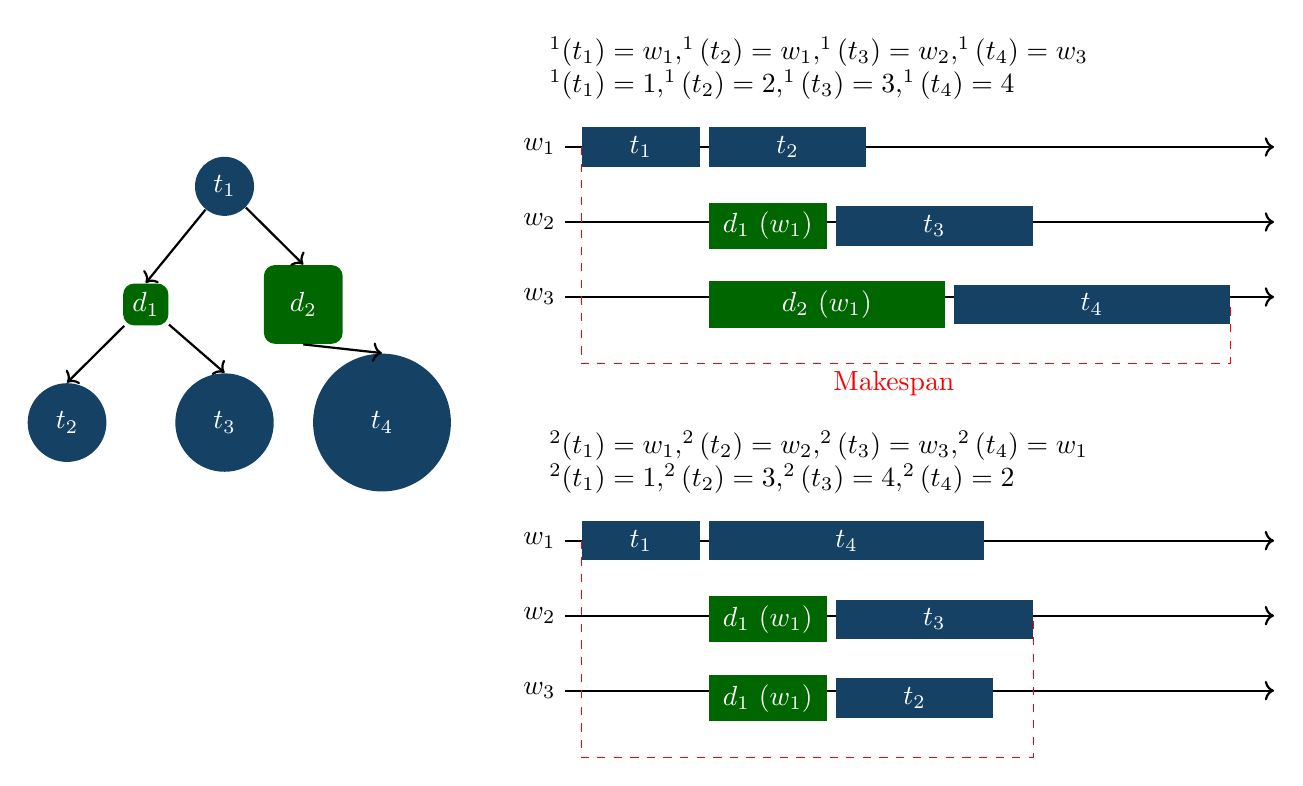
\begin{tikzpicture}
			\tikzmath{
				\tzerowidth = 15mm;
				\tonewidth = 20mm;
				\ttwowidth = 25mm;
				\tthreewidth = 35mm;
				\ozerowidth = 15mm;
				\oonewidth = 30mm;
			}
			\tikzset {
				taskstyle/.style={fill={rgb,255:red,21; green,66; blue,100}, text=white, draw=none},
				objstyle/.style={fill=black!60!green, text=white, draw=none},
			}

			% T1
			\node[task, taskstyle, minimum size=7.5mm] (t1) at (0, 0.5) {$t_1$};
			\node[data, objstyle, minimum size=5mm] (d1a) at (-1, -1) {$d_1$};
			\node[data, objstyle, minimum size=10mm] (d1b) at (1, -1) {$d_2$};
			\draw [arrow] (t1) edge (d1a.north) (t1) edge (d1b.north);

			% T2 and T3
			\node[task, taskstyle, minimum size=10mm] (t2) at (-2, -2.5) {$t_2$};
			\node[task, taskstyle, minimum size=12.5mm] (t3) at (0, -2.5) {$t_3$};
			\draw [arrow] (d1a) edge (t2.north) (d1a) edge (t3.north);

			% T4
			\node[task, taskstyle, minimum size=17.5mm] (t4) at (2, -2.5) {$t_4$};
			\draw [arrow] (d1b.south) edge (t4.north);

			% Move to the right to draw the timelines
			\tikzset{shift={(4,2)}}

			\node[anchor=west,align=left] at (0, 0) {
				$\scheduleworker^1(t_1) = w_1, \scheduleworker^1(t_2) = w_1, \scheduleworker^1(t_3) = w_2, \scheduleworker^1(t_4) = w_3$ \\
				$\scheduleorder^1(t_1) = 1, \scheduleorder^1(t_2) = 2, \scheduleorder^1(t_3) = 3, \scheduleorder^1(t_4) = 4$
			};

			\tikzset{shift={(0,-1)}}
			\node (tim1A) at (0, 0) {$w_1$};
			\draw[arrow] (tim1A.east) -- ++(9, 0);
			\node[below = 0.5 of tim1A.south] (tim1B) {$w_2$};
			\draw[arrow] (tim1B.east) -- ++(9, 0);
			\node[below = 0.5 of tim1B.south] (tim1C) {$w_3$};
			\draw[arrow] (tim1C.east) -- ++(9, 0);

			% Timeline 1, row 1
			\node[taskstyle, minimum width=\tzerowidth, right = 0.2 of tim1A.east] (tim1t0) {$t_1$};
			\node[taskstyle, minimum width=\tonewidth, right = 0.1 of tim1t0.east] (tim1t1) {$t_2$};

			% Timeline 1, row 2
			\node[objstyle, minimum width=\ozerowidth, below = 1 of tim1t1.west, anchor=west]
			(tim1o0) {$d_1$ ($w_1$)};
			\node[taskstyle, minimum width=\ttwowidth, right = 0.1 of tim1o0.east] (tim1t2) {$t_3$};

			% Timeline 1, row 3
			\node[objstyle, minimum width=\oonewidth, below = 1 of tim1o0.west, anchor=west]
			(tim1o1) {$d_2$ ($w_1$)};
			\node[taskstyle, minimum width=\tthreewidth, right = 0.1 of tim1o1.east]
			(tim1t3) {$t_4$};

			\draw[dashed, draw=red] (tim1t0.west) -- ++(0, -2.75) --
			([shift=({0,-0.75})]tim1t3.east) -- (tim1t3.east);

			\node[text=red] at (4.5, -3) {Makespan};

			% Move below to draw the timelines
			\tikzset{shift={(0,-4)}}

			\node[anchor=west,align=left] at (0, 0) {
				$\scheduleworker^2(t_1) = w_1, \scheduleworker^2(t_2) = w_2, \scheduleworker^2(t_3) = w_3, \scheduleworker^2(t_4) = w_1$ \\
				$\scheduleorder^2(t_1) = 1, \scheduleorder^2(t_2) = 3, \scheduleorder^2(t_3) = 4, \scheduleorder^2(t_4) = 2$
			};

			\tikzset{shift={(0,-1)}}
			\node (tim2A) at (0, 0) {$w_1$};
			\draw[arrow] (tim2A.east) -- ++(9, 0);
			\node[below = 0.5 of tim2A.south] (tim2B) {$w_2$};
			\draw[arrow] (tim2B.east) -- ++(9, 0);
			\node[below = 0.5 of tim2B.south] (tim2C) {$w_3$};
			\draw[arrow] (tim2C.east) -- ++(9, 0);

			% Timeline 2, row 1
			\node[taskstyle, minimum width=\tzerowidth, right = 0.2 of tim2A.east] (tim2t0) {$t_1$};
			\node[taskstyle, minimum width=\tthreewidth, right = 0.1 of tim2t0.east] (tim2t1)
			{$t_4$};

			% Timeline 2, row 2
			\node[objstyle, minimum width=\ozerowidth, below = 1 of tim2t1.west, anchor=west]
			(tim2o0) {$d_1$ ($w_1$)};
			\node[taskstyle, minimum width=\ttwowidth, right = 0.1 of tim2o0.east] (tim2t2) {$t_3$};

			% Timeline 2, row 3
			\node[objstyle, minimum width=\ozerowidth, below = 1 of tim2o0.west, anchor=west]
			(tim2o1) {$d_1$ ($w_1$)};
			\node[taskstyle, minimum width=\tonewidth, right = 0.1 of tim2o1.east] (tim2t3) {$t_2$};

			\draw[dashed, draw=red] (tim2t0.west) -- ++(0, -2.75) --
			([shift=({0,-1.75})]tim2t2.east) -- (tim2t2.east);
		\end{tikzpicture}
	}
	\caption{Simple task graph and two different schedules}
	\label{fig:scheduling-example}
\end{figure}

\vspace{2mm}Task scheduling is so crucial because it has a profound effect on the
efficiency of the whole workflow execution. We can observe that in~\Autoref{fig:scheduling-example}, which
shows a schedule for a simple task graph, and demonstrates how a trivial change in the schedule can
severely affect the resulting makespan. The figure contains a task graph with four tasks and two
data objects. The size of the circles is proportional to the execution duration of the tasks and
the size of the rounded rectangles is proportional to the size of the data objects.

Let us assume that we want to schedule this task graph in a computational environment with three
workers $(w_1, w_2, w_3)$. Two different schedules for this situation are shown in the figure.
Schedule $S^1$ assigns tasks $t_1$ and $t_2$ to
worker $w_1$, task $t_3$ to worker $w_2$ and
task $t_4$ to worker $w_3$, while schedule $S^2$
assigns tasks $t_1$ and $t_4$ to worker $w_1$,
task $t_3$ to worker $w_2$ and task $t_2$ to
worker $w_3$. The timelines shows the execution of tasks (blue rectangles) and
the network transfers of data objects between workers (green rectangles) for each individual
worker. It is clear that with $S^2$, the task graph will be computed faster than
with $S^1$, even though the only difference between the two schedules is that the
tasks $t_2$ and $t_4$ were swapped between workers
$w_1$ and $w_3$. Note that the timeline assumes that a worker
can overlap the computation of a task with the transfer a data object to another worker over the
network, which is commonly supported by existing task runtimes.

Optimal scheduling of tasks to workers is an NP-hard~\cite{Ullman1975} problem even for the
most basic scenarios, when the exact execution duration of each task is known, and even if we do
not consider the duration of transferring data between workers over a network. Task runtimes thus
resort to various heuristics tailored to their users' needs. Some classic task scheduling
heuristics and their comparisons can be found in~\cite{estee,hlfet1974,kwok1998benchmarking,hagras2003static,wang2018list}. \Autoref{ch:estee}
provides a comprehensive survey of various task scheduling algorithms.

%Scheduling heuristics have to take many factors into consideration when deciding on which worker
%should a task be executed:
%
%\begin{description}[wide=0pt]
%	\item[Resource requirements] The scheduler should respect all resource requirements specified by tasks. The runtime thus has to
%		observe the dynamically changing available resources of each worker and schedule tasks accordingly,
%		to uphold their requirements. This can be challenging especially in the presence of complex
%		resource requirements.
%	\item[Data transfer cost] If the runtime operates within a distributed cluster, one of the most important scheduling aspects
%		that it needs to consider is the transfer cost of data between workers over the network. All
%		benefits gained by computing a task on another worker to achieve more parallelization might be lost
%		if it takes too much time to send the data (task outputs) to that worker.
%
%		The scheduler thus has to carefully balance the communication-to-computation ratio, based on the
%		available network bandwidth, sizes of outputs produced by tasks and the current utilization of
%		workers.
%	\item[Scheduling overhead] The overhead of generating the schedule itself also cannot be underestimated. As was already
%		stated, computing an optimal solution quickly is infeasible, but even heuristical approaches can
%		have wildly different performance characteristics. Producing a lower quality schedule sooner,
%		rather than a higher quality schedule later, can be sometimes beneficial.
%	\item[Memory consumption] It is desirable to execute as many tasks in parallel on a given worker (with respect to its
%		available parallelism), to speed up the completion of the whole workflow. However, the scheduler
%		should also balance the number of concurrently executing tasks according to the total amount of
%		memory that they consume. In general, it is difficult to predict for how long will a task execute,
%		and how much (peak) memory will it consume. When a task executes longer than expected, the workflow
%		will still be computed, it will just take more time. But when a task uses more memory than
%		expected, or the scheduler puts too many tasks on a worker at the same time, then the worker might
%		run out of memory and crash. If this happens repeatedly, it can stall or completely stop the
%		execution of the workflow. For memory-intensive workflows, the runtime should assign fewer tasks at
%		the same time to a single worker, or reduce overall memory consumption in some other way, e.g.\ by
%		keeping less cached data objects in the worker's memory.
%\end{description}

\section*{Summary}
This chapter has provided a basic definition of the most important terms related to task-based
programming models that will be used throughout this chapter. It has introduced the notion of task
graphs, tasks, data objects, resource requirements, workers, task runtimes and task scheduling.

The following chapter will focus on describing what challenges are faced by users and task runtimes
when they execute task graphs on \gls{hpc} clusters.


\chapter{Task graph challenges in HPC}
\label{ch:challenges}
Task-based programming is quite popular and useful, as it provides a simple way to define complex
workflows which can then be executed in a wide range of environments, ranging from consumer
laptops, through cloud deployments, to distributed HPC clusters. However, as any programming model,
it also has some disadvantages and problems. It is crucial to understand these limitations in order
to design approaches for overcoming them.

This chapter thus describes various challenges and requirements of this programing model, both in
terms of efficient and scalable execution, and in terms of the offered productivity and ergonomics.
It focuses specifically on challenges and requirements required by HPC use-cases, which introduce a
unique set of constraints stemming both from the inherent complexity of HPC software and hardware
and also from the sheer computational scale required to efficiently utilize HPC resources.

In addition to the challenges, we will also mention various desired properties and features which
should be offered by task runtimes in order to either support the mentioned requirements or to
alleviate the mentioned problems.

\section{Allocation manager}
The vast majority of HPC systems use some kind of allocation manager (such as
PBS\slash{}Torque~\cite{pbs} or Slurm~\cite{slurm}) to
facilitate submission of computations, resource management and user
accounting~\cite{slurm-schedmd}. To perform any computation through an allocation manager, the
user has to submit an \emph{allocation}\footnote{The term \emph{job} is also commonly used for the concept of HPC computational
requests. However, we will reserve this term for a different concept described later in the thesis and use the term
\emph{allocation} for HPC computational requests.}, a computational request
that states (amongst other things) how many nodes they want to allocate and what is the expected
maximum duration of their computation. The allocation is then submitted into a
\emph{queue} and starts to execute only once there are enough free computational
resources. Allocation managers are used to provide fair access to HPC resources, to avoid their
oversubscription and also to handle accounting of computation. They tend to have fairly strict
limits on the number of allocations that users can submit and the number of nodes that they can
have reserved for their allocations at any given time.

Since users have to create computational requests through the allocation manager, and thus they
cannot simply execute their task graphs directly on an HPC cluster, a natural question arises --
how to map tasks (or task graphs) to HPC allocations in order to efficiently utilize HPC resources?
Several ways of performing this mapping are described below, however all of them come with
significant disadvantages.

\subsection*{Execute the whole task graph in a single allocation} This is the simplest case. If the
task graph does not have a large number of tasks, or if it can be executed quickly, it could be
submitted within a single allocation. This approach is quite simple for the user, since they just
execute the task graph using some task runtime in the same way as they would on a cluster without
an allocation manager or on a personal computer. The only difference is that they have to define
and submit an allocation that will bootstrap the computation.

However, since allocations are bound both by node count and time limits, this approach will only be
usable for rather small task graphs. Indeed, if the computation is short, it might not even make
sense to use an HPC cluster to compute it. A more realistic scenario is that even if an individual
task graph can be executed quickly, users might want to execute many such task graphs (for example
to execute many experiments with different parametrizations). This situation can be seen as a
special case of a large task graph that consists of many disjoint components (smaller task
subgraphs). In this case, it will typically not be possible to execute all such task graphs inside
a single allocation.

\subsection*{Execute each task as an individual allocation} From a certain point of view, HPC
allocation managers can also be viewed as task runtimes that operate on a very coarse level --
their tasks being allocations that potentially span hundreds of nodes, run for days or even longer
and consist of many different program executions. Ideally, there would be no difference between an
allocation manager and a task runtime, and users would just be able to construct an arbitrarily
granular task graph and execute it directly on an HPC cluster in a straightforward way.

While this approach can certainly look tempting, in practice it is not always feasible to use the
currently popular allocation managers (Slurm and PBS) in this way, because they operate on a level
that is far too coarse for complex fine-grained task graphs. They tend to have large overhead per
each allocation, which can be several orders of magnitude larger than for typical task runtimes
(e.g.\ seconds vs milliseconds). Furthermore, they seldom allow the user to create more than a few
hundreds of allocations at the same time, both to provide fairness and also because they simply
cannot scale to such an number of allocations. And their support for expressing dependencies
between the individual tasks (allocations) is also quite basic.

It should be noted that even though there is definitely room for improving the scheduling
performance of HPC allocation managers, some of their complexity and performance limitations are
inherent. They have to provide accurate accounting, handle robust and secure cleanup of
allocations, take care of user and process isolation, ensure user fairness and many other things.
Many of these responsibilities are out of scope for task runtimes, which enables them to achieve
higher performance.

Another problem is node granularity. For ``small'' tasks that only use e.g.\ a few cores, users
would like to schedule and execute multiple tasks on a single node at the same time, to leverage
the available hardware resources efficiently. While allocation managers are able to create
allocations that require only a fraction of a node, this functionality tends to be sometimes
disabled. Either for security reasons, because tasks from multiple users can then execute on the
same node in parallel, and thus user isolation is reduced, or for performance reasons, because the
overhead of scheduling a large number of allocations (in theory many allocations per each node) can
become unmanageable for the allocation manager~\cite{it4i_node_scheduling_policy}. When the manager is set
up in a way that a single allocation has to span at least a (complete) single node, it can lead to
wasted resources if a single task cannot leverage the whole computational node.

Last, but not least, another reason why users might not want to use the allocation manager directly
as a task runtime is that it is useful to debug and prototype task graphs in a small-scale scenario
(e.g.\ locally, on a personal computer), before executing it on a large-scale HPC system. However,
it can be quite challenging for users to deploy systems like PBS or Slurm locally. Therefore, they
would need to use a different task runtime when executing the task graph locally and on the target
HPC platform, which is not very practical.

The mentioned issues create a certain dichotomy between the coarse-grained focused allocation
manager and more fine-grained focused task runtimes, and instead of facilitating simple workflow
execution on HPC clusters, it can create a barrier for users. Users that want to execute a task
graph on an HPC system thus usually use a separate task runtime (e.g.\
Dask~\cite{dask}) rather than using the allocation manager directly. Instead of
building a task graph of the whole computation and executing it with a single command, they have to
think about will they reconcile the coarse-grained nature of allocations with the fine-grained
nature of tasks. In practice, this means that they have to partition the tasks of their workflows
into allocations. As we have discussed above, if the whole task graph can be executed within a
single allocation, this is typically not an issue. However, when users need to create multiple
allocations, this process can be quite cumbersome.

\subsection*{Split the task graph into a smaller number of allocations}
This is the ultimate approach that task graph users will probably sooner or later converge to, once
their task graph becomes sufficiently complex. When the task graph does not fit within a single
allocation, and its tasks are too fine-grained for the overhead caused by the allocation manager,
the graph has to be partitioned into smaller parts which will then be executed in individual
allocations by independent instances of some task runtime.

This process is not straightforward, especially if users have to perform the partitioning manually.
Graph partitioning itself is a notoriously difficult problem that is
NP-hard~\cite{graph_partitioning}\todo{Ada: Is this OK?}, and it is thus difficult to decide
beforehand how exactly should the task graph be split into allocations. Furthermore, if the
partitioning of tasks into allocations is performed only once, before the computation begins, then
it might lead to suboptimal hardware utilization, as tasks will not be load balanced across
allocations, even if multiple allocations run concurrently.

In addition to partitioning the task graph, further code infrastructure might have to be
implemented, outside the boundaries of the task-based programming model. As an example, the
intermediate results of computed tasks of a partitioned subgraph might have to be stored (to some
storage system) before the corresponding allocation ends, and the results from multiple allocations
then have to be merged together. To robustly handle tasks that fail or to support adding new tasks
while a task graph is already executing, additional code might be needed to periodically submit new
allocations for tasks that have not been successfully finished yet, until the whole task graph is
computed. This reduces the ergonomics of using task graphs, because it basically forces the user to
reimplement part of the task runtime behavior on top of the allocation manager, to overcome its
limitations.

\vspace{5mm}
The gap between allocation managers and task runtimes creates a certain disconnect for users
attempting to scale their task graph computation. Running on a personal computer tends to be quite
simple. After that, moving to an HPC cluster and executing the entire task graph inside a single
allocation is also quite straightforward. But once the task graph has to be partitioned into
multiple allocations, the simple abstraction of implicitly parallel task graphs that can be
executed with a single command quickly falls apart, as the user has to perform a lot of additional
work to make this scenario execute efficiently.

Ideally, users would not have to think about the allocation manager; they should be able to
construct a task graph and execute it directly on an HPC cluster in a straightforward way, by
letting some tool perform the partitioning and load balancing across allocations automatically for
them. This could be achieved either by adding support for executing fine-grained task graphs to
allocation managers or by integrating task runtimes with allocation managers to provide transparent
execution of task graphs on HPC systems.

\section{Cluster heterogeneity}
Even though task graphs are designed to be portable and ideally should not depend on any specific
execution environment, for certain types of tasks, we need to be able to describe at least some
generic environment constraints. For example, when a task executes a program that leverages the
CUDA\todo{explain} framework, which is designed to be executed on a graphics
accelerator, it has to be executed on a node that has a GPU available, otherwise it will simply not
work.

It should thus be possible for an HPC task to define \emph{resource requirements}, which specify
resources that have to be provided by an environment that will execute such task. These
requirements can be quite diverse. For example, a requirement could be the number of cores (some
tasks can use only a single core, some can be multithreaded), the amount of available main memory,
a minimum duration required to execute the task or (either optional or required) presence of an
accelerator like a GPU or an FPGA\@. In order to remain portable and independent of a specific
execution environment, these requirements should be abstract and describe general, rather than
specific, types of resources.

The challenge related to resource requirements of HPC tasks specifically is the diverse hardware
present in modern HPC clusters, which have started to become increasingly heterogeneous in recent
years. This trend can be clearly seen in the TOP500 list of most powerful
supercomputers~\cite{top500analysis}. Individual cluster nodes contain varying amounts and
types of cores and sockets, main memory, NUMA nodes or accelerators like GPUs or FPGAs. Since HPC
software tries to leverage all these modern HPC hardware features, this complexity is also
propagated to tasks and their resource requirements, which can become relatively complex.

Some types of tasks might require a combination of several requirements, for example two GPUs,
sixteen cores and 32 GiB of main memory. Some tasks are designed in a way that allows them to
leverage an open-ended range of resources, e.g.\ a task might require four cores, but if more are
available, it could use as many as possible. Furthermore, some tasks might even support several
variants of requirements, for example a task might either use four cores and a single GPU (if there
is one available), or it could use more cores (and no GPU) to offset the absence of an accelerator.

A resource requirement that is fairly specific to HPC systems is the requirement of using multiple
nodes per single task. This requirement is necessary for programs that are designed to be executed
in a distributed fashion, such as programs using MPI, which are quite common in HPC. This
requirement is not supported in many task runtimes, because their programming model assumes that a
task performs an atomic computation that executes on a single node. The use-case of tasks using
multiple nodes is discussed in more detail later in this chapter.

To support the mentioned scenarios, task runtimes should allow users to specify arbitrarily
fine-grained and abstract resource requirements for each task. They should also allow users to
attach resources that will satisfy these requirements to each individual instance of an execution
environment that will execute the tasks. Runtimes should also be able to take these requirements
into account when scheduling, both to make sure that the requirements are upheld, and also to
utilize the available hardware effectively.

\section{Data transfers}
After a task is computed, it can produce various data outputs, standard error or output streams,
files created on the disk or data objects that are then passed as inputs to dependent tasks. There
are many ways of storing and transferring these outputs. Some task frameworks store task outputs on
the filesystem, since it is relatively simple to implement, and it provides support for basic data
resiliency out-of-the-box.

HPC nodes might not contain any local disks, but instead use shared filesystems accessed over a
network. While this can be seen as an advantage, since with a shared filesystem it is much easier
to share task outputs amongst different workers, it can also be a severe bottleneck. Shared
networked filesystems can suffer from quite high latency, and accessing them can consume precious
network bandwidth that is also used e.g.\ for managing computation (sending commands to workers) or
for direct worker-to-worker data exchange. Furthermore, data produced in HPC computations can be
quite large, and thus storing it to a disk can be a bottleneck even without considering networked
filesystems.

These bottlenecks can be alleviated by transferring task outputs directly between workers over the
network (preferably without accessing the filesystem in the fast path), by streaming outputs
between tasks without the need to store them or by leveraging RAM disks~\cite{hyperloom}.
Making use of HPC specific technologies, such as MPI or InfiniBand, could be also worthwhile to
leverage the very fast interconnects available in HPC clusters.

Data outputs produced by tasks tend to be considered immutable in existing task runtimes, since a
single output can be used as an input to multiple tasks, and these might be executed on completely
different computational nodes. A problem that can arise with this approach is that if the data
outputs are large, but the computation within tasks that work with the data is short, the
serialization overhead (or even memory copy overhead, if the dependent task is executed on the same
node) can dominate the execution time. Such use-cases can be solved with stateful data management,
for example in the form of \emph{actors}, which can be considered stateful tasks that
operate on a single copy of some large piece of data.

\section{Fault tolerance}
Fault tolerance is relevant in all distributed computing environments, but HPC systems have
specific requirements in this regard. As was already mentioned, computational resources on HPC
clusters are provided through allocation managers. Computing nodes allocated by these managers are
provided only for a limited duration, which means that for long-running task graphs, some nodes
will disconnect and new nodes will appear dynamically during the execution of the task graph.
Furthermore, since the allocations go through a queue, it can take some time before new
computational resources arrive, therefore the task graph can remain in a paused state, where no
tasks are being executed, for potentially long periods of time.

It is important for task runtimes to be prepared for these situations; they must handle node
disconnections gracefully, even if a task was being executed on a node that disconnects, and they
should be able to restart previously interrupted tasks on newly arrived workers. In general, in HPC
scenarios, worker instability and frequent disconnects should be considered the norm, not just a
rare edge case.

\section{Multi-node tasks}
Many existing HPC applications are designed to be executed on multiple (potentially hundreds or
even thousands) nodes in parallel, using e.g.\ MPI libraries or other communication frameworks.
Multi-node execution could be seen as a special resource requirement, which states that a task
should be executed on multiple workers at once.

Support for multi-node tasks affects many design areas of a task runtime:
\begin{description}
	\item[Scheduling] When a task requires multiple nodes for execution and not enough nodes are available at a given
		moment, the scheduler has to decide on a strategy that will allow the multi-node task to execute.
		If it was constantly trying to backfill available workers with single-node tasks, the multi-node
		tasks could be starved.

		The scheduler might thus have to resort to keep some nodes idle for a while to enable the
		multi-node task to start as soon as possible. Another approach could be to interrupt the currently
		executing tasks and checkpoint their state to make space for a multi-node task, and then resume
		their execution once the multi-node task finishes.

		In a way, this decision-making already has to be performed on the level of individual cores even
		for single-node tasks, but adding multiple nodes per task makes the problem much more difficult.
	\item[Data transfers] It is relatively straightforward to express data transfers between single-node tasks in a task
		graph, because they naturally correspond to dependencies (edges) between the tasks. With multi-node
		tasks, the data distribution patterns become more complex, for example data can be replicated from
		a single node to multiple nodes when a multi-node task starts or gathered (reduced) from multiple
		nodes to a single node when such task finishes.

		When several multi-node tasks depend on one another, the task runtime should be able to exchange
		data between them in an efficient manner. This might require some cooperation with the used
		communication framework (e.g.\ MPI) to avoid needless repeated serialization and deserialization.
	\item[Fault tolerance] When a node executing a single-node task crashes or disconnects from the runtime, its task can be
		rescheduled to a different worker. In the case of multi-node tasks, failure handling requires more
		communication and is generally more complex. When a task is executing on four nodes and one of them
		fails, the runtime has to make sure that the other nodes will be notified of this situation, so
		that they can react accordingly (either by finishing the task with a smaller number of nodes or by
		also failing immediately).
\end{description}

To enable common HPC usecases, task runtimes should be able to provide some support for multi-node
tasks and allow them to be combined with single-node tasks. Advanced multi-node task support could
be provided e.g.\ by offering some kind of integration with MPI or similar common HPC technologies.

\section{Scalability}
The sheer scale of HPC performance (node count, core count, network interconnect bandwidth) opens
up opportunities for executing large scale task graphs, but that in turn presents unique challenges
for task runtimes. Below you can find several examples of bottlenecks that might not matter in a
small computational scale, but that can become problematic in the context of HPC-scale task graphs.

\begin{description}
	\item[Task graph materialization] Large computations might require building massive task graphs that contain millions of tasks. The
		task graphs are typically defined and built outside the task runtime itself, for example on the
		login nodes of computing clusters or on client devices (e.g.\ laptops), which can provide only
		relatively low performance. It can be quite slow to build, serialize and transfer such graphs over
		the network to the task runtime. This can create a bottleneck even before any task is executed.
		This has been identified as an issue in existing task runtimes~\cite{dask-client-perf}.

		In such case, it can be beneficial to provide an API for defining task graphs in a symbolic way,
		for example by representing a potentially large group of similar tasks by a single entity. Such
		symbolic graphs could then be sent to the runtime in a compressed form and re-materialized only at
		the last possible moment. In an extreme form, the runtime could operate on such graphs in a fully
		symbolic way, without ever materializing them.
	\item[Communication overhead] Scaling the number of tasks and workers will necessarily put a lot of pressure on the communication
		network, both in terms of bandwidth (sending large task outputs between nodes) and latency (sending
		small management messages between the scheduler and the workers). Using HPC technologies, such as
		MPI or a lower-level interface like RDMA (Remote Direct Memory Access), could provide a non-trivial
		performance boost in this regard.

		As we have demonstrated in~\cite{pspin, spin2}, in-network computing, an active area of
		research, can be also used to optimize various networking applications by offloading some
		computations to an accelerated NIC (network interface controller). This approach could also be
		leveraged for task runtimes, for example by reducing the latency of management messages between the
		scheduler and workers or by increasing the bandwidth of large data exchanges amongst workers, by
		moving these operations directly onto the network card.
	\item[Runtime overhead] As we have shown in~\cite{rsds}, task runtimes with a centralized scheduler have to
		make sure that their overhead remains manageable. Even with an overhead of just
		$1ms$ per task, executing a task graph with a million tasks would result in
		total accumulated overhead of twenty minutes! Our results indicate that increasing the performance
		of the central scheduling and management component of a task runtime can have a large positive
		effect on the overall time it takes to execute the whole task graph.

		However, the performance of the central server cannot be increased endlessly, and from some point,
		using a centralized architecture, which is common to task runtimes, itself becomes a bottleneck.
		Even if the workers exchange large output data directly between themselves, any single, centralized
		component may become overloaded simply by coordinating and scheduling the workers.

		In that case, a decentralized architecture could be leveraged to avoid the reliance on a central
		component. Such a decentralized architecture can be found e.g.\ in Ray~\cite{ray}.
		However, to realize the gains of a decentralized architecture, task submission itself has to be
		decentralized in some way, which might not be a natural fit for common task graph workflows. If all
		tasks are generated from a single component, the bottleneck will most likely remain even in an
		otherwise fully decentralized system.
\end{description}

\section{Iterative computation}
A natural way of executing task graphs is to describe the whole computation with a single task
graph, submit the graph to the task runtime and wait until all the tasks are completed. However,
there are some computations that need a more iterative approach. Training a machine learning model
can be stopped early if the loss is no longer decreasing. A chemical or physical simulation is only
considered completed once a desired accuracy has been reached, which might take a previously
unknown number of steps. These scenarios and many others like them, are quite common in HPC use
cases.

To support iterative computation, task runtimes should allow the user to stop the execution of a
task graph (or its subgraph) once a specific condition is met, and also to add new tasks to the
task graph in a dynamic fashion, if it is discovered that more iterations are needed.

\section{Summary}
Even though more HPC use-cases and oddities could always be found, it is already clear from the
mentioned challenges that HPC use-cases that leverage task graphs can contain a lot of complexity.
It could be possible to add support for some mentioned requirements to existing task runtimes,
which are described in the next section. However, the described challenges are so diverse and
complex that a dedicated approach which considers them holistically could provide a better solution
that would avoid both ergonomics and performance from being compromised.

The aforementioned requirements will serve as a basis for further research in the proposed thesis.
The goal of the thesis is to design approaches for executing task graphs on HPC systems that take
the aforementioned requirements into account. These approaches will leverage the
\hyperqueue{} task runtime, which is described further in
Chapter~\ref{ch:hyperqueue}.


\chapter{State of the art}
\label{ch:sota}
- pydra

% TODO: https://docs.google.com/document/d/1C43tAGIRqy1hDHajRTiyM2q_TeihJwH0e66ASeGOwfU/edit#heading=h.rzzu2ckt23ak


\chapter{Task scheduler analysis}
\label{ch:estee}
% Algoritmy: https://docs.google.com/document/d/1cDg8dV4Rso5sAE2gYkBPsJ8a_dMLqA8MHRR1ZvceWZM/edit#heading=h.7z19cc4fgwy4
%TODO: Our results indicate that network models used by many previous works might produce results
%that are off by an order of magnitude in comparison to a more realistic model. Additionally, we
%show that certain implementation details of scheduling algorithms which
%are often neglected can have a large effect on the scheduler’s performance, and they
%should thus be described in great detail to enable proper evaluation.

Task scheduling is one of the most important responsibilities of a task runtime in terms of
performance, because the quality of the generated schedule has a large effect on the total makespan
of the task graph execution and also on the achieved hardware utilization of worker nodes. It is
crucial for the scheduler to be able to distribute the tasks amongst all available worker nodes to
achieve as much parallelization as possible, without the induced network communication and task
management becoming a bottleneck. Unfortunately, optimal task scheduling is a very difficult
problem, which is NP-hard even in the simplest cases~\cite{Ullman1975}, and there is thus no
single scheduling algorithm that could quickly provide an optimal schedule for an arbitrary task
graph.

There are many factors that affect the execution properties of task graphs and that pose some form
of a challenge to task schedulers. The execution environment (e.g.\ a distributed cluster) can have
varying amounts of nodes with heterogeneous hardware resources, and complex network topologies that
can have a non-trivial effect on the latency and bandwidth of messages sent between the workers and
the scheduler, and thus in turn also on the overall performance of the task graph execution. Task
graphs can be structured arbitrarily, with large amounts of different kinds of tasks with diverse
execution characteristics and resource requirements.

Furthermore, task graph execution might not be deterministic, and the scheduler has to work with
incomplete information and react to events that dynamically occur during task execution and that
cannot be fully predicted before the task graph has started executing. The communication network
can be congested because of unrelated computations running concurrently on the cluster, tasks can
also be slowed down by congested hardware resources that can be highly non-trivial to model (e.g.\
\gls{numa} effects), and they can also sometimes fail unpredictably and must be
re-executed. Even the duration of each task, which is perhaps the most crucial property of a task
coveted by the scheduler, is usually not known beforehand, and the most the scheduler knows about
is either an estimate from the task graph author or a running average based on historical
executions of similar tasks, both of which can be inaccurate.

In theory, all these factors should be taken into account by task scheduling algorithms. In
practice, it is infeasible to have a completely accurate model of the entire cluster, operating
system, task implementations, networking topology etc. Therefore, task schedulers omit some of
these factors to provide reasonable runtime performance. They rely on various heuristics and make
different trade-offs that make them better suited for specific types of task graphs and execution
environments. These heuristics can suffer from non-obvious edge cases that produce bad quality
schedules or from low runtime efficiency, which can in turn erase any speedup gained from producing
a higher quality schedule.

For \gls{hpc} use-cases, the performance and quality of task scheduling is even more
important, since the scale and heterogeneity of task graphs used in \gls{hpc}
provides a challenge for the scheduler. \gls{hpc} clusters also tend to provide
advanced network topologies with low latency and high bandwidth~\cite{dragonfly,slimfly}, which
offer the scheduler more leeway to create sophisticated schedules leveraging large amounts of
network communication, which would otherwise be infeasible on clusters with slower networks.

To better understand the behaviour and performance of various scheduling algorithms, we have
performed an extensive analysis of several task scheduling algorithms in
\emph{Analysis of workflow schedulers in simulated distributed environments}~\cite{estee}. The two main contributions of this work are as
follows:
\begin{enumerate}
	\item We have created an extensible, open-source simulator of task graph execution, which allows users to
	      easily implement their own scheduling algorithms and compare them, while taking into account
	      various factors that affect task scheduling.
	\item We have benchmarked several task schedulers from existing literature under various conditions,
	      including factors affecting scheduling that have not been explored so far, like the minimum delay
	      between invoking the scheduler or the amount of knowledge about task durations available to the
	      scheduler, and evaluated the suitability of the individual algorithms for various types of task
	      graphs. All parts of the benchmark suite in an open and reproducible form. This includes the task
	      graphs, all source code for the schedulers and the simulation environment and also all benchmark
	      scripts.
\end{enumerate}

Various descriptions of schedulers, task graphs and other parts of the simulator and the benchmark
configuration used in this chapter were adapted from our publication~\cite{estee}.

\workshare{I have collaborated on this work with Ada Böhm and Vojtěch Cima, we have all contributed to it equally. Source code contribution statistics for
\estee{} can be found on GitHub\footnoteurl{https://github.com/it4innovations/estee/graphs/contributors}.}

\section{Task graph simulator}
\label{sec:estee-simulator}
To analyze scheduling algorithms, some form of an environment for executing task has to be used.
One possibility would be to use an actual distributed cluster, and implement multiple schedulers
into an existing task runtime. However, this approach can be expensive, both computationally
(executing a large number of task graphs with various configurations would consume a lot of cluster
computational time) and implementation-wise (adapting existing runtimes to different scheduling
algorithms is challenging). Therefore, task graph scheduling surveys tend to use some form of a
simulated environment, which simulates selected properties of a distributed cluster, and allows
comparing the performance of multiple scheduling algorithms (or other factors of a task runtime)
with smaller accuracy, but at a fraction of the  cost.

Many task scheduler surveys have been published over the years~\cite{hlfet1974, kwok1998benchmarking, hagras2003static, sinnen2005, wang2018list}, yet it is
difficult to reproduce and extend these results without having access to the exact source code used
to implement the schedulers and the simulation environment used in these surveys. As we will show
in the following chapter, the performance of scheduling algorithms can be highly affected by
seemingly trivial implementation details, and having access only to a high-level textual
description or pseudocode of a scheduling algorithm does not guarantee that it will be possible to
reproduce it independently with the same performance characteristics. This makes it challenging to
compare results between different simulation environments.

Apart from the environments used in existing surveys, there are also more general task simulation
environments. DAGSim~\cite{dagsim} offers a framework for comparing scheduling
algorithms, and compares the performance of a few algorithms, but does not provide its
implementation, which makes it difficult to reproduce or extend its results.
SimDAG~\cite{simdag} is a task graph simulator focused on \gls{hpc}
use-cases built on top of the SimGrid~\cite{simgrid} framework. It allows relatively
simple implementation of new task scheduling algorithms, however it does not support any task
resource requirements (e.g.\ the number of used \gls{cpu} cores).

In addition to simply comparing the performance of different schedulers, our goal was also to test
two factors that affect scheduling, which we have not seen explored in detail in existing works.
Namely, we wanted to examine the effects of \gls{msd}, the delay between two
invocations of the scheduler and \emph{information mode}, the amount of knowledge of task durations
that is available to the scheduler. These factors will be described in detail in the following
section. The existing simulation environments that we have evaluated did not have support for these
factors, and it would be non-trivial to add support for them.

To summarize, our goal was to have a simulation environment that would be open-source, to provide
full reproducibility, would support basic task resource requirements and would enable us to examine
the two mentioned factors that affect scheduling. To fulfill these goals, we have implemented a new
task graph simulation framework called \estee{}. It is an \mbox{MIT-licensed}
open-source tool~\cite{estee_github} written in Python that provides an experimentation testbed
for task runtime and scheduler developers and researchers. It is flexible; it can be used to
define a cluster of workers, connect them together using a configurable network model, implement a
custom scheduling algorithm and test its performance on arbitrary task graphs, with support for
specifying required \gls{cpu} core counts for individual tasks. At the same time, it
comes ``battery-included'', and contains baseline implementations of several task schedulers from
existing literature and also a task graph generator that can be used to generate randomized graphs
with properties similar to real-world task graphs.

\subsection{Architecture}
\Autoref{fig:estee-architecture} shows the architecture of \estee{}. The core of the
tool is the Simulator component, which uses discrete event simulation to simulate the execution of
a task graph. It manages task lifetime, queries the Scheduler component for task-to-worker
assignments (schedules) and then assigns the tasks to their corresponding workers. The Worker
component then simulates task execution, and also uses the provided network model to simulate
exchanges of data (task outputs) between the individual workers in the simulated cluster.

\begin{figure}
	\centering
	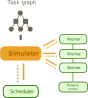
\includegraphics[scale=0.35]{estee/estee-architecture}
	\caption{\estee{} architecture}
	\label{fig:estee-architecture}
\end{figure}

\estee{} provides abstract interfaces for the task scheduler, the worker and the
network model (which simulates network communication and congestion). Users can thus easily provide
their own implementations of these interfaces, and in turn override both the behavior of the
scheduler and of the cluster and its network topology.

One of our goals for \estee{} was to make it very easy to write new scheduling
algorithms and make the scheduler approachable for other researchers that might want to experiment
with task schedulers. That was also one of the motivations why we decided to create
\estee{} in Python, which facilitates experimentation. \Autoref{lst:estee-example} shows
an example of a task graph simulation that demonstrates the simplicity of defining task graph
simulation using \estee{}. The output of the simulation is both the makespan (the
duration it took to execute the task graph) and also a detailed trace that can be used to visualize
the individual task-to-worker assignments and task execution time spans.

\begin{listing}
	\begin{minted}[fontsize=\small]{python}
# Create task graph containing 3 tasks
# (each task runs for 1s and requires 1 CPU)
#
#     t0
#     | (50MB output)
#    / \
#  t1   t2
tg = TaskGraph()
t0 = tg.new_task(duration=1, cpus=1, output_size=50)
t1 = tg.new_task(duration=1, cpus=1)
t1.add_input(t0)
t2 = tg.new_task(duration=1, cpus=1)
t2.add_input(t0)

# Create a task scheduler
scheduler = BlevelGtScheduler()

# Define cluster with 2 workers (1 CPU each)
workers = [Worker(cpus=1) for _ in range(2)]

# Define MaxMinFlow network model (100MB/s bandwidth)
netmodel = MaxMinFlowNetModel(bandwidth=100)

# Run simulation, returns the makespan in seconds
simulator = Simulator(tg, workers, scheduler, netmodel, trace=True)
makespan = simulator.run()
print(f"Task graph execution makespan = {makespan}s")
    \end{minted}
	\caption{Simple task graph simulation example using \estee{}}
	\label{lst:estee-example}
\end{listing}

\estee{} supports general task graphs represented by a \gls{dag}.
Each task has an associated duration, and can contain multiple outputs (data objects), each with an
associated size. It can also specify how many cores does it require, to model the common
requirement of executing multithreaded functions and programs on modern \gls{hpc}
machines. The used model of a task graph corresponds precisely to the task graph definition
contained in \Autoref{ch:taskgraphs}.

\subsection{Communication model}
Some previous scheduler surveys assume that the time to transfer a data object from one worker to
another depends merely on the size of the data object, and not on other factors, such as current
network utilization or interference~\cite{tang2010list,yao2013task,wang2018list,kwok1996dynamic}. This is an unrealistic assumption, as
the latency and bandwidth of actual computer networks is affected (amongst other things) by other
communication happening concurrently on the same network. Moreover, a real worker implementation
would download more than a single data object simultaneously, which further affects the transfer
durations, because the worker's bandwidth will be shared by multiple network tranfers. We will use
the term \emph{communication model} and \emph{network model} interchangeably in this chapter.

We provide a more realistic network model that simulates full-duplex communication between workers,
where the total (data object) upload and download bandwidth of each worker is limited. The sharing
of bandwidth between worker connections is modeled by the
\emph{max-min fairness model}~\cite{bertsekas_1992}. Max-min fairness provides a bandwidth allocation
for each worker. If an allocation of any participant is increased, then we necessarily have to
decrease the allocation of some other participant with an equal or smaller allocation. When a data
object transfer starts or finishes, the data flow between workers is recomputed immediately, thus
we neglect the fact that it may take some time for the bandwidth to fully saturate.

%TODO: odkomentovat?
%This model is not as accurate as e.g.\ packet-level simulation implemented in some other
%simulators~\cite{simgrid}, but it is a notable improvement over the naive model.

To provide a baseline that corresponds to the naive model described above, which has been used in
several previous works, \estee{} also implements a \emph{simple} network
model.

It is possible to choose an arbitrary network bandwidth amount for a given simulation for any used
networking model.

\subsection{Scheduler parameters}
%TODO: odstranit konec této  věty?
\estee{} implements support for two parameters that can affect scheduler
performance, and which we have not seen examined in detail in existing literature:
\begin{description}
	\item[Minimal scheduling delay] Non-trivial schedulers create task assignments continuously during task graph execution, based on
		the current worker load and task completion times. That means that they are not invoked only once,
		but rather the task runtime invokes them repeatedly, to ask them to produce assignments for tasks
		that are (or soon will be) ready to be executed at any given point in time.

		It then becomes an important for a task runtime to decide when exactly should it invoke the
		scheduler. It could try to make a scheduling decision every time a task is finished; however, in
		practice there is often an upper bound on the number of scheduler invocations per second. It might
		be introduced artificially, to reduce the scheduling overhead, or it might be caused by a software
		or hardware limitation (e.g.\ messages containing task updates cannot be received more often).
		Furthermore, creating a new schedule after each task status change might not be optimal. The
		runtime can also accumulate changes for a short time period, and then provide the scheduler with a
		batch of status updates. While this increases the latency of task assignments, it can give the
		scheduler more context to work with, when it decides how it should assign tasks to workers.

		To test our hypothesis that the scheduler invocation rate can affect its performance, we introduce
		a parameter called \emph{Minimal scheduling delay (\acrshort{msd})}, which forces a minimal delay between two scheduler
		invocations, i.e.\ the scheduler cannot be invoked again before the at least
		\gls{msd} time units have elapsed since its previous invocation.
	\item[Information mode] Many existing task scheduler descriptions assume that the duration of each task (and the size of
		each data object) is known in advance. However, this assumption is very seldom upheld when
		executing real-world task graphs. Tasks are usually specified using arbitrary functions or binary
		invocations, and it is difficult to estimate their duration up front. Task runtimes thus
		have to work with completely missing information about task durations, depend on potentially
		imprecise user estimates, or calculate their own estimates based on historical task execution data.
		Task benchmarks usually use simulated task durations, which are provided to the scheduler. However,
		this might not realistically represent the scheduler's behavior for actual task graphs, for which
		we usually do not know task durations precisely.

		We use a parameter called \emph{Information mode (imode)}, which controls the amount of knowledge the
		scheduler has of the duration of tasks. It can be set to one of the following values:
		\begin{description}
			\item[\emph{exact}] The scheduler has access to the exact duration of each task and the exact size of each data object
				in the whole task graph.
			\item[\emph{user}] The scheduler has access to user-defined estimations for each task in the task graph. These
				estimations are sampled from a random distribution that corresponds to a specific kind of task
				within the workflow. For example, in a task graph that performs three kinds of tasks (e.g.\
				preprocessing, computation and postprocessing), each kind of task would have its own distribution.
				We have categorized the tasks of task graphs that we have used for scheduler benchmarks described
				in~\Autoref{sec:estee-benchmarks} manually, to simulate a user that has some knowledge of the task graph
				that they are trying to compute and is able to provide some estimate of task durations and data
				object sizes.
			\item[\emph{mean}] The scheduler has only access to the mean duration of all tasks and the mean size of all data
				objects in the executed task graph. This simulates a situation where a similar task graph is
				executed repeatedly, and thus there is at least some aggregated information about the task
				properties available from an earlier run.
		\end{description}
		Another possible mode to consider could be to not provide the scheduler with any task durations nor
		data object sizes in advance. This behaviour would in fact correspond closely to a real-world
		execution of a task graph, where we usually do not know these task properties a priori. However, it
		is challenging to use this approach when benchmarking schedulers. Scheduler implementations are
		typically described with the assumption that task durations are known, and the scheduling
		algorithms are often fundamentally based on calculations that make use of them.

		If we took away this information, it would make many schedulers very sensitive to an initial
		estimate of the durations and sizes (and the ratio between them, which influences decisions whether
		to move data objects between workers to enable more parallelization). This estimate strongly
		influences the behavior of schedulers, and if task durations would be completely unknown, the
		behavior of different schedulers could converge and be heavily affected by the estimate.

		It is also unclear how to even compute such an estimate, which would have to be chosen almost
		arbitrarily. Therefore, we propose to use the \emph{mean} mode instead of not providing
		the scheduler with any information. This assumes that even if the scheduler knows nothing in
		advance, it could always monitor the durations and sizes of finished tasks gradually and such
		monitored values would converge to the mean. In practice, this would take some time, while in our
		environment the schedulers know about the mean in advance. Nevertheless, as was already mentioned,
		we can often get a reasonable estimate of the mean durations based on previous executions of
		similar workflows.
\end{description}

%TODO: uncomment?
%\subsection{Worker inner scheduler}
%Since each worker has to keep track of its running tasks, manage resources, and
%handle data object transfers, it becomes relatively complex. In practice, the global
%scheduler cannot micromanage each worker because this approach could not scale
%to a larger number of workers. Therefore, we model a situation where each
%worker has its own inner scheduler. We call it \emph{w-scheduler} and we
%reserve the word ``scheduler'' for the global scheduler that assigns tasks to
%workers.
%
%The w-scheduler is not a subject of study in this work, hence we are going to
%fix one particular worker scheduler and execute all experiments with it.
%The implementation is inspired by the worker implementation used in
%HyperLoom~\citep{hyperloom} and Rain. It is described in Appendix~A.

\subsection{Schedulers}
\label{subsec:estee-schedulers}
There are many task scheduling approaches, and an enormous number of various task scheduling
algorithms. We have implemented a set of task schedulers that are representatives of several common
scheduling approaches, inspired by a list of schedulers from a survey performed by Wang and
Sinnen~\cite{wang2018list}. We have included several representatives of the simplest and
perhaps most common list-scheduling approach, but also schedulers that use work-stealing or genetic
algorithms.

List-scheduling is an intuitive approach where the scheduler sorts tasks (into a list) based on
some priority criteria, and then repeatedly chooses the task with the highest priority, and assigns
it to a worker (which is selected by another heuristic).

Below is a list of schedulers that we have implemented and benchmarked\footnote{The labels of the individual schedulers correspond to labels used in charts that will be presented
in~\Autoref{sec:estee-benchmarks}.}:
\noindent\textbf{blevel}\quad \gls{hlfet}~\cite{hlfet1974} is a
foundational list-based scheduling algorithm that prioritizes tasks based on their
\emph{b-level}. B-level of a task is the length of the longest path from the task to any
leaf task (in our case the length of the path is computed using durations of tasks, without taking
data object sizes into account). The tasks are scheduled in a decreasing order based on their
b-level.

\noindent\textbf{tlevel}\quad
Smallest Co-levels First with Estimated Times~\cite{kwok1999static} is similar to
\gls{hlfet}, with the exception that the priority value computed for each task (which
is called \emph{t-level} here) is computed as the length of the longest path from any
source task to the given task. This value corresponds to the earliest time that the task can start.
The tasks are scheduled in an increasing order based on their t-level.

\noindent\textbf{dls}\quad
Dynamic Level Scheduling~\cite{sih1993compile} calculates a dynamic level for each task-worker
pair. It is equal to the static b-level lessened by the earliest time that the task can start on a
given worker (considering necessary data transfers). In each scheduling step, the task-worker pair
that maximizes this value is selected.

\noindent\textbf{mcp}\quad
The Modified Critical Path~\cite{wu1990hypertool} scheduler calculates the ALAP
(as-late-as-possible) time for each task. This corresponds to the latest time the task can start
without increasing the total schedule makespan. The tasks are then ordered in ascending order based
on this value, and scheduled to the worker that allows their earliest execution.

\noindent\textbf{etf}\quad
The ETF (Earliest Time First) scheduler~\cite{hwang1989scheduling} selects the task-worker pair that
can start at the earliest time at each scheduling step. Ties are broken by a higher b-level
precomputed at the start of task graph execution.

\noindent\textbf{genetic}\quad
This scheduler uses a genetic algorithm to schedule tasks to workers, using the mutation and
crossover operators described in~\cite{omara2009genetic}. Only valid schedules are considered, if
no valid schedule can be found within a reasonable number of iterations, a random schedule is
generated instead.

\noindent\textbf{ws}\quad
This is an implementation of a simple work-stealing algorithm. The default policy is that each task
that is ready to be executed (all its dependencies are already computed) is always assigned to a
worker where it can be started with a minimal transfer cost. The scheduler then continuously
monitors the load of workers. When a worker starts to starve (and thus does not have enough tasks
to compute), then a portion of tasks assigned to other workers is rescheduled to the starving
worker.

In addition to these schedulers, we have also implemented several naive schedulers, which serve as
a baseline for scheduler comparisons.

\noindent\textbf{single}\quad
This scheduler simply assigns all tasks to a single worker (it selects the worker with the most
cores). The resulting schedule never induces any data transfers between workers, and does not take
advantage of any parallelism between workers.

\noindent\textbf{random}\quad
This scheduler simply assigns each task to a random worker using a \gls{prng} engine.

We have tried to implement the mentioned list-based schedulers (\emph{blevel},
\emph{tlevel}, \emph{dls}, \emph{mcp}, \emph{etf})
as closely as possible to their original description. These list-based algorithms mostly focus on
selecting the next task to schedule, but an important question (that comes up during their
implementation) is to what worker should the selected task be scheduled. The algorithm description
often mention assigning the task to a worker that allows the earliest start time of the task. While
that is surely a reasonable heuristic, it is not clear how exactly should such a worker be found,
because the exact earliest start time often cannot be determined precisely in advance, since its
calculation might encompass network transfers whose duration is uncertain by nature. This seemingly
simple implementation detail is crucial for impementing the scheduler, and it should be included in
the description of all scheduling algorithms.

\estee{} implementations of these schedulers use a simple estimation of the earliest
start time, which is based on the currently executing and already scheduled tasks of a worker, and
an estimated network transfer cost based on uncontended network bandwidth (in other words, the
\emph{simple} network model is used for the scheduler's estimation of the network
transfer cost).

In order to test our hypothesis that the worker selection approach is important and affects
the scheduler's behavior, we have also created extended versions of the \emph{blevel},
\emph{tlevel} and \emph{mcp} schedulers. These modified versions use a
worker selection heuristic called ``greedy transfer``. We have not applied this heuristic to other
list-based schedulers, where it would fundamentally change their behavior.

%TODO: reword this? better differentiate between the naive heuristic and greedy-transfer?
The greedy transfer heuristic assigns the selected task to a worker that has a sufficient number of
free cores on which the task may be executed and that requires the minimal data transfer (sum over
all sizes of data objects that have to be transferred to that worker). It also adds support for
clusters where some machines have a different number of cores than others. When a task
$t$ that needs $c$ cores cannot be scheduled because of an
insufficient number of free cores, the list scheduling continues by taking another task in the list
instead of waiting for more free cores. This task will only consider workers that have less than
$c$ cores. This allows to schedule more tasks while it does not modify the
priority of tasks because $t$ cannot be scheduled on such workers anyway. Note
that when all workers have the same number of cores, the behavior is identical to ordinary list
scheduling.

\subsection{Task graphs}
To facilitate task scheduler experiments, \estee{} contains a task graph generator,
which is able to generate parametrized instances of various categories of task graphs. Graphs from
each category can be generated using several parameters that affect their resulting size and shape.
To increase the variability of the graphs, properties like task durations or data object sizes are
sampled from a normal distribution. Below is a description of the three categories of task graphs
that can be generated:

%TODO: explain fork-join?
\vspace{1mm}\noindent\textbf{elementary}\quad This category contains trivial graph
shapes, such as tasks with no dependencies or simple fork-join graphs. These graphs can test the
behavior of scheduler heuristics on basic task graph building blocks that frequently form parts of
larger workflows. Examples of these graphs can be seen in \Autoref{fig:estee-elementary-shapes}.

\vspace{1mm}\noindent\textbf{irw}\quad This generator creates graphs that are
inspired by real-world workflows, such as machine learning cross-validations or map-reduce
computations.

\vspace{1mm}\noindent\textbf{pegasus}\quad This category is derived from graphs
created by the Synthetic Workflow Generators~\cite{pegasusgraphs}. The generated graphs
correspond to the \emph{montage}, \emph{cybershake}, \emph{epigenomics},
\emph{ligo} and \emph{sipht} Pegasus workflows. The graphs have been
extended with additional properties required for testing information modes (notably expected task
durations and data object sizes for the \emph{user} information mode).

\section{Task scheduler benchmarks}
\label{sec:estee-benchmarks}
We have performed an extensive analysis of the performance of several task scheduling algorithms on
various task graphs using the \estee{} simulator. The aim of the analysis was to
explore the behavior of various schedulers in a complex simulation environment. In addition to
comparing the schedulers amongst each other, we also wanted to test how does their performance
differ between various communication models and scheduler parameters.

Note that since the used simulation environment is focused on simulating different task graph
schedules and network transfers, and it does not model the actual execution of the scheduler nor
the task runtime in a cycle-accurate way, the term \emph{scheduler performance} refers to the simulated
makespan of task graphs executed using schedules provided by the given scheduler. Our goal is thus
to compare how quickly would a given task graph be fully computed on a cluster (and a network
model) while being scheduled by different scheduling algorithms, while also taking into account the
mentioned scheduler parameters.

\subsection{Benchmark configuration}
This section describes the cluster, scheduler and task graph configurations that we have used for
our benchmarks.

\begin{description}
	\item[Task graphs] The \estee{} graph generators were used to generate a collection of task graphs that
		were used in the benchmarks. The properties of all used graphs are summarized in
		Table~\ref{tab:estee-graph-properties}. The generated task graph dataset is available as a reproducible
		artifact~\cite{estee_graphs}.
	\item[Schedulers] We have benchmarked all schedulers described in~\Autoref{sec:estee-simulator}. Schedulers that use the
		greedy transfer heuristic are labeled with a \emph{-gt} suffix in benchmark results.
	\item[Scheduler parameters] To evaluate the effect of minimal scheduling delay, we have used a baseline value of zero, where
		the scheduler is invoked immediately after any task status update, and then a delay of 0.1, 0.4,
		1.6 and 6.4 seconds. In the cases where \gls{msd} is non-zero, we have also added a 50
		milliseconds delay before sending the scheduler decision to workers, to simulate the time taken by
		the scheduler to produce the schedule. For experiments that do not focus on \gls{msd},
		we always use an \gls{msd} of 0.1 seconds and the 50 milliseconds computation delay.
		To evaluate information modes, we have used the \emph{exact}, \emph{user} and
		\emph{mean} imodes. For experiments that do not focus on imodes, we always use the
		\emph{exact} mode.
	\item[Network models] The simple (labeled \emph{simple}) and max-min (labeled \emph{max-min}) network
		models were used, with bandwidth speeds ranging from 32 MiB/s to 8 GiB/s. For experiments that do
		not focus on the network model (e.g.\ when imodes are compared), we always use the
		\emph{max-min} network model.
	\item[Clusters] We have used the following five cluster (worker) configurations (where $w \times c$ means
		that the cluster has $w$ workers and each worker has $c$
		cores):  8$\times$4, 16$\times$4, 32$\times$4,
		16$\times$8, 32$\times$16.
\end{description}

%TODO: fix cut task graph
\begin{figure}
	\centering
	\begin{subfigure}{.2\textwidth}
		\centering
		\includegraphics[width=.8\textwidth]{imgs/estee/shapes/plain}
		\caption{}
		\label{fig:tg-plain}
	\end{subfigure}%
	\begin{subfigure}{.2\textwidth}
		\centering
		\includegraphics[width=.8\linewidth]{imgs/estee/shapes/fork}
		\caption{}
		\label{fig:tg-fork}
	\end{subfigure}
	\begin{subfigure}{.2\textwidth}
		\centering
		
\includegraphics[width=.8\linewidth]{imgs/estee/shapes/fork2}
		\caption{}
		\label{fig:tg-fork2}
	\end{subfigure}
	\begin{subfigure}{.2\textwidth}
		\centering
		
\includegraphics[width=.8\linewidth]{imgs/estee/shapes/v}
		\caption{}
		\label{fig:tg-v}
	\end{subfigure}
	\\
	\begin{subfigure}{.2\textwidth}
		\centering
		
\includegraphics[width=.8\linewidth]{imgs/estee/shapes/w}
		\caption{}
		\label{fig:tg-w}
	\end{subfigure}
	\begin{subfigure}{.2\textwidth}
		\centering
		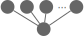
\includegraphics[width=.8\linewidth]{imgs/estee/shapes/merge}
		\caption{}
		\label{fig:tg-merge}
	\end{subfigure}
	\begin{subfigure}{.2\textwidth}
		\centering
		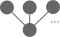
\includegraphics[width=.8\linewidth]{imgs/estee/shapes/merge-triplets}
		\caption{}
		\label{fig:tg-merge-triplets}
	\end{subfigure}
	\begin{subfigure}{.2\textwidth}
		\centering
		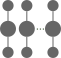
\includegraphics[width=.8\linewidth]{imgs/estee/shapes/triplets}
		\caption{}
		\label{fig:tg-triplets}
	\end{subfigure}
	\\
	\begin{subfigure}{.2\textwidth}
		\centering
		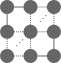
\includegraphics[width=.8\linewidth]{imgs/estee/shapes/grid}
		\caption{}
		\label{fig:tg-grid}
	\end{subfigure}
	\begin{subfigure}{.2\textwidth}
		\centering
		\includegraphics[width=.8\linewidth]{imgs/estee/shapes/splitters}
		\caption{}
		\label{fig:tg-splitters}
	\end{subfigure}
	\begin{subfigure}{.2\textwidth}
		\centering
		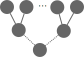
\includegraphics[width=.8\linewidth]{imgs/estee/shapes/conflux}
		\caption{}
		\label{fig:tg-conflux}
	\end{subfigure}
	\begin{subfigure}{.2\textwidth}
		\centering
		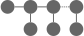
\includegraphics[width=.8\linewidth]{imgs/estee/shapes/fern}
		\caption{}
		\label{fig:tg-fern}
	\end{subfigure}

	\caption{Task graph shapes in the \emph{elementary} data set}
	\label{fig:estee-elementary-shapes}
\end{figure}

\begin{table}
	\centering
	\begin{tabular}{l|lrrrr|T}
		\toprule
		Graph            & D & \#T & \#O   & TS     & LP  & \normalsize{Description}     \\
		\midrule
		plain1n          & e & 380 & 0     & 0.00   & 1   & Independent tasks;
		normally distributed durations (Fig.~\ref{fig:tg-plain})                         \\
		plain1e          & e & 380 & 0     & 0.00   & 1   & Independent tasks;
		exponentially distributed durations (Fig.~\ref{fig:tg-plain})                    \\
		plain1cpus       & e & 380 & 0     & 0.00   & 1   & Independent tasks with
		varying core requirements (Fig.~\ref{fig:tg-plain})                              \\
		triplets         & e & 330 & 220   & 17.19  & 3   & Task triplets; middle
		task requires 4 cores (Fig.~\ref{fig:tg-triplets})                               \\
		merge\_neighb.   & e & 214 & 107   & 10.36  & 2   & Merge of adjacent
		task pairs (Fig.~\ref{fig:tg-w})                                                 \\
		merge\_triplets  & e & 148 & 111   & 10.77  & 2   & Merge of task
		triplets (Fig.~\ref{fig:tg-merge-triplets})                                      \\
		merge\_sm-big    & e & 240 & 160   & 7.74   & 2   & Merge of two
		results (0.5 MiB and 100 MiB data objects) (Fig.~\ref{fig:tg-v})                 \\
		fork1            & e & 300 & 100   & 9.77   & 2   & Tasks with a pair of
		consumers each consuming the same output (Fig.~\ref{fig:tg-fork})                \\
		fork2            & e & 300 & 200   & 19.53  & 2   & Tasks with a pair of
		consumers each consuming different output (Fig.~\ref{fig:tg-fork2})              \\
		bigmerge         & e & 321 & 320   & 31.25  & 2   & Merge of a large
		number of tasks (variant of Fig.~\ref{fig:tg-merge})                             \\
		duration\_stairs & e & 380 & 0     & 0.00   & 1   & Independent
		tasks; task durations range from 1 to 190 s (Fig.~\ref{fig:tg-plain})            \\
		size\_stairs     & e & 191 & 190   & 17.53  & 2   & 1 producer 190
		outputs / 190 consumers; sizes range from 1 to 190 MiB                           \\
		splitters        & e & 255 & 255   & 32.25  & 8   & Binary tree of
		splitting tasks (Fig.~\ref{fig:tg-splitters})                                    \\
		conflux          & e & 255 & 255   & 31.88  & 8   & Merging task pairs
		(inverse of \emph{splitters}) (Fig.~\ref{fig:tg-conflux})                        \\
		grid             & e & 361 & 361   & 45.12  & 37  & Tasks organized in a 2D grid
		(i.e. \emph{splitters} followed by \emph{conflux}) (Fig.~\ref{fig:tg-grid})
		\\
		fern             & e & 401 & 401   & 11.11  & 201 & Long task sequence with
		side tasks (Fig.~\ref{fig:tg-fern})                                              \\ \hline
		gridcat          & i & 401 & 401   & 115.71 & 4   & Merge of pairs of 300 MiB
		files                                                                            \\
		crossv           & i & 94  & 90    & 8.52   & 5   & Cross validation             \\
		crossvx          & i & 200 & 200   & 32.66  & 5   & Several instances of cross
		validation                                                                       \\
		fastcrossv       & i & 94  & 90    & 8.52   & 5   & Same as \emph{crossv}
		but tasks are $50\times$ shorter                                                 \\
		mapreduce        & i & 321 & 25760 & 439.06 & 3   & Map-reduce pattern           \\
		nestedcrossv     & i & 266 & 270   & 28.41  & 8   & Nested cross
		validation                                                                       \\ \hline
		montage          & p & 77  & 150   & 0.21   & 6   & Montage workflow
		from Pegasus                                                                     \\
		cybershake       & p & 104 & 106   & 0.84   & 4   & Cybershake
		workflow from Pegasus                                                            \\
		epigenomics      & p & 204 & 305   & 1.36   & 8   & Epigenomics
		workflow from Pegasus                                                            \\
		ligo             & p & 186 & 186   & 0.11   & 6   & Ligo workflow from
		Pegasus                                                                          \\
		sipht            & p & 64  & 136   & 0.12   & 5   & Sipht workflow from
		Pegasus                                                                          \\
		\bottomrule
	\end{tabular}\\
	\vspace{2mm}
	D = Dataset (e = elementary, i = irw, p = pegasus); \#T = Number of tasks; \#O = Number of outputs;
	TS = Sum of all output object sizes (GiB); LP = longest oriented path in the graph

	\caption{Scheduler benchmark task graph properties}
	\label{tab:estee-graph-properties}
\end{table}

\subsection{Evaluation}
This section discusses selected noteworthy results of the described benchmarks. Completele
benchmark results and overview charts can be found in~\cite{estee}. The benchmarking
environment, input task graph datasets, all used benchmark configurations, results and charts are
also freely available as reproducible artifacts~\cite{estee_results} for further examination.

The benchmarks were executed on the clusters of the IT4Innovations supercomputing
centre~\cite{it4i}. The actual characteristics of the cluster hardware is not
important, because all benchmarks were executed using the \estee{} simulator, so the
benchmark results do not depend on the used hardware. Each benchmark that was non-deterministic in
any way (e.g.\ because it used a pseudo-random number generator) was executed twenty times. Unless
specified otherwise, the individual experiments were performed with the default benchmark
configuration that uses the \emph{max-min} network model, the \emph{exact}
information mode and a Minimal Scheduling Delay of 0.1s.

\subsubsection*{Random scheduler}

%TODO: chart does not start at zero
\begin{figure}
	\centering
	\includegraphics[width=\textwidth]{imgs/estee/charts/random-scheduler}\\
	{\small x axis: bandwidth [MiB/s]; y axis: makespan [s]; row: cluster}
	\caption{Performance of the \emph{random} scheduler}
	\label{fig:estee-chart-random-scheduler}
\end{figure}

Given the fact that task scheduling is an NP-hard problem, it would seem that a random scheduling
approach should produce unsatisfying results. We thus wanted to examine how does a completely
random scheduler hold up against more sophisticated approaches. \Autoref{fig:estee-chart-random-scheduler} compares
the simulated makespan durations of the \emph{random} scheduler vs. two other schedulers
that are quite competitive (\emph{blevel-gt} and the work-stealing \emph{ws}
scheduler) on several task graphs.

While there are indeed cases where random scheduling falls short (for example on the
cross-validation \emph{crossv} task graph, or in situations with many workers and a slow
network), in most cases its performance is similar to other schedulers, and it even surpasses
them in a few situations! Its performance gets better with increasing worker count and network
speed. This makes sense, because if there are enough workers and the network is fast enough to
overcome the cost of exchanging many data objects between them, the specific assignment of tasks
between workers becomes less important. As long as the scheduler is able to keep the workers busy
(which can be ensured even by a random schedule, for some task graphs), then the resulting
performance is reasonable.

We have been able to validate these results in~\cite{rsds}, where we have shown that as
the worker count becomes larger, scheduling decisions can in some cases become less important, and
other factors (like runtime performance of the task runtime) might start to dominate the overall
task graph execution cost. This will be described in more detail in \Autoref{ch:rsds}.

\subsubsection*{Worker selection strategy}

\begin{figure}
	\centering
	\includegraphics[width=0.8\textwidth]{imgs/estee/charts/gt-scheduler}\\
	{\small x axis: bandwidth [MiB/s]; y axis: makespan [s]; row: cluster}
	\caption{Comparison of worker selection strategy}
	\label{fig:estee-chart-gt-scheduler}
\end{figure}

As was explained in~\ref{subsec:estee-schedulers}, the descriptions of several schedulers that we have
implemented in~\estee{} do not specify the concrete strategy for selecting a worker
that can start executing a given task as soon as possible. Yet, as we can see in
\Autoref{fig:estee-chart-gt-scheduler}, this implementation detail is crucial. This chart shows the performance of
two scheduling algorithms (\emph{blevel} and \emph{mcp}), each in two
variants, with the simple selection strategy and with the greedy transfer strategy (the used worker
selection strategy was the only difference between the simple and the \emph{-gt}
suffixed variants).

It can be seen that there is a large difference between these two strategies. In fact, the results
suggest that in these specific scenarios, the worker selection strategy had a larger effect on the
overall performance than the used scheduling (task selection) algorithm, as the variants using
greedy transfer were highly correlated.

\subsubsection*{Network models}

\begin{figure}
	\centering
	\includegraphics[width=\textwidth]{imgs/estee/charts/irw-32x4-netmodel-score}\\
	{\small x axis: bandwidth [MiB/s]; y axis: makespan normalized to average
	of makespan of \emph{simple} model; row: scheduler; cluster $32x4$}
	\caption{Comparison of \emph{max-min} and \emph{simple} network models
		(\emph{irw} dataset)}
	\label{fig:estee-chart-irw-netmodel}
\end{figure}

\begin{figure}
	\centering
	\includegraphics[width=\textwidth]{imgs/estee/charts/pegasus-32x4-netmodel-score}
	\\ {\small x axis: bandwidth [MiB/s]; y axis: execution makespan normalized
	to average of makespan of \emph{simple} model; row: scheduler, cluster
	$32x4$}
	\caption{Comparison of \emph{maxmin} and \emph{simple} network models
		(\emph{pegasus} dataset)}
	\label{fig:estee-chart-pegasus-netmodel}
\end{figure}

\Autoref{fig:estee-chart-irw-netmodel} demonstrates how does the used network model affect simulated task
graph makespans for a selected set of task graphs and schedulers, using task graphs from the
\emph{irw} dataset on the $32x4$ cluster with 32 workers. The Y axis
is normalized with respect to the average makespan of simulations performed with the
\emph{simple} network model.

It is clear that especially for slower network bandwidths, the naive \emph{simple} model
often underestimates the resulting makespan. This is caused by the fact that it does not take
network contention into account at all, which causes the overall network transfer duration
estimation to be overly optimistic. As network bandwidth goes up, the difference is reduced, since
there is less overall contention and the transfers are faster in general.

The makespans of simulations with these two network models are sometimes up to an order of
magnitude apart. This is quite significant, because the difference between the performance of
schedulers (with a fixed network model) is otherwise usually within a factor of two, which was
demonstrated both by our other results and in~\cite{wang2018list}. The gap between the two
network models depends heavily on the used task graph. For task graphs from the Pegasus dataset,
the difference was much smaller, as can be seen in~\Autoref{fig:estee-chart-pegasus-netmodel}.

\subsubsection*{Minimal scheduling delay}

\begin{figure}
	\centering
	\includegraphics[width=0.8\textwidth]{imgs/estee/charts/irw-32x4-schedtime-score}\\
	{\small x axis: bandwidth [MiB/s]; y axis: makespan normalized to
	$\gls{msd}=0$}
	\caption{Comparison of \gls{msd}; cluster 32x4}
	\label{fig:estee-chart-irw-msd}
\end{figure}

In \Autoref{fig:estee-chart-irw-msd}, we can observe the effect of \gls{msd} on graphs from the
\emph{irw} dataset, with the $32x4$ cluster configuration. The Y axis
is normalized with respect to the configuration where \gls{msd} is zero. The results
show that the effect of \gls{msd} is relatively limited. There does not seem to be
any clear correlation or pattern that would suggest that a smaller \gls{msd}
consistently improves performance of a scheduler. Although, interestingly a higher
\gls{msd} value caused several makespan improvements, especially on the
\emph{gridcat} task graph.

This is (again) an example of the non-trivial effect of scheduler heuristics. Increasing the
\gls{msd} leads to batching effect, where the scheduler is allowed to make decisions
less often, but it has knowledge of more task events (that have arrived during the delay) during
each decision. Whether this helps its performance, or hurts it, depends on the specific scheduler
implementation and the task graph that it executes.

\subsubsection*{Information modes}

\begin{figure}
	\centering
	\includegraphics[width=\textwidth]{imgs/estee/charts/irw-32x4-imode-score}\\
	{\small x axis: bandwidth [MiB/s]; y axis: makespan normalized to
	\emph{exact}
	imode; row: scheduler; cluster $32x4$}
	\caption{Comparison of information modes (\emph{irw} dataset)}
	\label{fig:estee-chart-irw-imode}
\end{figure}

%\begin{figure}
%	\centering
%	\includegraphics[width=0.8\textwidth]{imgs/estee/charts/elementary-32x4-imode-score}\\
%	{\small x axis: bandwidth [MiB/s]; y axis: makespan normalized to
%	\emph{exact} average; row: scheduler; cluster $32x4$}
%   \caption{Comparison of information modes (\emph{elementary} dataset)}
%   \label{fig:estee-chart-elementary-imode}
%\end{figure}

\Autoref{fig:estee-chart-irw-imode} compares makespans of several scheduler and task graph combinations
from the \emph{irw} dataset on a $32x4$ cluster, with different
information modes being used. The results are normalized to the mean makespan of the default
\emph{exact} information mode. In general, the effect of information modes is more
significant than the effect of the Minimal Scheduling Delay.

An intuitive expectation would be that with more precise task duration information, the scheduler
will be able to produce a shorter makespan, and this is indeed what happens in several cases, e.g.\
on the \emph{mapreduce} and \emph{nestedcrossv} task graphs with the
\emph{blevel-gt} scheduler, where the makespan is up to 25\% longer when task durations are
not exactly known.

However, there are also opposite cases, for example the \emph{dls} and
\emph{mcp} schedulers produce better results on several task graphs when they take
only the \emph{mean} task duration into account. This further shows the effect of
scheduler heuristics, which can produce worse results even when presented with more accurate data
input (and vice versa).

One factor that makes it more difficult for the scheduler to accurately estimate the network
transfer durations and thus make optimal use of the knowledge of task durations is that with the
max-min network model, the scheduler knows only a lower bound on the communication costs, even if
it knows the exact data size in advance. While it has access to the maximum bandwidth of the
network, it does not know the current (and most importantly, future) network utilization, thus it
only has a crude estimation of the real transfer duration.

\subsection{Validation}
It is challenging to validate the performance of different task schedulers in actual task
runtimes. Schedulers of existing runtime tend to be deeply integrated within them, in order to be
as performant as possible. That makes it difficult, or even infeasible, to replace the scheduling
algorithm without also modifying large parts of the runtime. Furthermore, some scheduling
approaches might not even be compatible with the architecture of the runtime as a whole. For
example, work-stealing schedulers perform a lot of communication between the server and the workers
(potentially even between the workers themselves), and if the runtime does not implement the
necessary infrastructure for facilitating these communication patterns, then implementing a
work-stealing scheduler into such a runtime might amount to rewriting it from scratch.

In order to at least partially validate our simulation results, we have decided to use a modified
version of the \dask{}~\cite{dask} task runtime as a validation
framework. Apart from validating results from the \estee{} simulations, we have also
used this modified version of \dask{} to perform other experiments and benchmarks
that are described in \Autoref{ch:rsds}, which also depicts the architecture of
\dask{} and our performed modifications in detail.

\dask{} is written in Python, which makes it relatively easy to modify and patch.
It uses a work-stealing scheduler by default, and even though it is relatively deeply integrated
within the Dask runtime, we were able to implement three simple alternative scheduling algorithms
into it~\footnote{The modified version of \dask{} with these implemented schedulers can be found at
\url{https://github.com/Kobzol/distributed/tree/simple-frame-sched}.}, which correspond as closely as possible to the
\emph{random}, \emph{blevel} and \emph{tlevel} schedulers from
\estee{}. The default work-stealing scheduler was compared with our work-stealing
implementation of the \emph{ws} scheduler.

Apart from implementing new schedulers into \dask{}, there were several issues that
we had to solve to make sure that he comparison between the simulated and the real environment is
as fair and accurate as possible.

The absolute makespans of task graphs simulated by \estee{} and task graphs executed
by \dask{} cannot be compared directly, because there are many aspects of the
operating system, network, implementation of \dask{} itself and system noise that
\estee{} can not fully simulate. Therefore, since the primary goal of our task
scheduler experiments was to compare the relative performance of individual schedulers, we have
decided to compare the relative makespans normalized to a reference scheduler
(\emph{blevel}), to test if the makespan ratios between the schedulers is similar in
simulation and in real execution.

In the scheduler benchmarks, we have used many task graphs generated by the \estee{}
task graph generator. However, it would not be possible to perfectly replicate task durations of
these generated graphs in \dask{}. Therefore, we have approached this problem from
the other direction. We have executed several task graphs in \dask{}, and recorded
their execution traces, so that we would have a completely accurate representation of all the
executed task durations and data object sizes, which we could then accurately replicate in the
simulated \estee{} environment. The recorded task graphs are described in
\Autoref{ch:rsds} and also in~\cite{rsds}. We have executed these task graphs
with a $24x2$ cluster (24 cores on two nodes), and performed each execution and
simulation three times.

\begin{figure}
	\centering
	\includegraphics[width=\textwidth]{imgs/estee/charts/estee-validation}\\
	{\small x axis: scheduler; y axis: performance relative to \emph{blevel}}
	\caption{Scheduler performance relative to \emph{blevel} in \dask{} and \estee}
	\label{fig:estee-validation}
\end{figure}

\Autoref{fig:estee-validation} shows the results of the validation comparison for three selected
task graphs\footnote{Extended validation results can be found in~\cite{estee}.}. The performance of each scheduler was normalized to the
makespan of the \emph{blevel} scheduler within the same environment (either
\estee{} or \dask{}). Note that the relative ratios were centered
around zero by subtracting $1$ from them, to focus on the relative differences.
For example, if a task graph took $100s$ to execute in \dask{} with
the \emph{blevel} scheduler, but $110s$ with the \emph{ws}
scheduler, the ratio of the \emph{ws} scheduler would be $0.1$. If
the simulation was perfect, the two columns for each scheduler would have the same height.

The first chart shows a situation where changing the scheduler resulted in large changes in
makespans, and \estee{} was able to accurately simulate these changes, and reflect
the results measured in \dask{}. The second chart demonstrates a situation where
all schedulers produce similar makespans, therefore in this case the scheduling algorithm does not
seem to be that important. \estee{} was again able to estimate that the differences
between schedulers will be small. In the third chart, we see that \estee{} was
systematically overestimating the makespans of all three schedulers (with respect to the reference
scheduler). The most important difference was in the \emph{ws} scheduler, where the
simulated result claims that it is slower than \emph{blevel}, while in reality it was
slightly faster. The work-stealing implementation in \dask{} is complex, and in
this case it was able to outperform \emph{blevel} in a way that \estee{}
was not able to simulate.

To summarize the average error of the simulated results, we took the relative makespans of the
individual schedulers w.r.t.\ the reference \emph{bevel} scheduler, and calculated the
difference between the executed and simulated relative makespan. The geometric mean of these
differences across all measured benchmarks was $0.0347$, which suggests that the
differences between the execution and simulation were relatively small, and the simulated makespans
were usually within just a few percent of the actual makespan duration.

\section*{Summary}
We have implemented a set of well known scheduling heuristics, prepared a benchmark dataset
containing task graphs of different types and scales and designed a simulation environment for task
scheduler experimentation. We have conducted a series of fully reproducible benchmarks using that
environment, in which we have analyzed the effect of network models, minimal scheduling delays,
information modes and worker selection strategy on the behaviour of the implemented schedulers, and
also compared their relative performance.

Our attempts to implement existing scheduling algorithms in \estee{} and reproduce
the results of previous scheduler benchmarks have shown that various implementation details which
are often missing from the algorithm's description (like the precise worker selection strategy) can
have a large effect on the final performance of the scheduler. Furthermore, we have been able to
confirm our hypothesis that the naive network model used in several existing works can result in
very inaccurate simulation results.

Combined with the fact that the source code of many published scheduling algorithms or surveys is
not open-source, it is difficult (even nigh impossible) to accurately reproduce their performance
results. We have tried our best to make all available source-code, benchmark datasets and the
results of our experiments public, to make them easy to reproduce and thus avoid this issue.

Our analysis has shown that despite its simplicity, the foundational \gls{hlfet}
algorithm~\cite{hlfet1974} produces high quality schedules in various scenarios and should
thus serve as a good baseline scheduler for task runtimes.

We have also demonstrated that even a completely random scheduler can be competitive with other
scheduling approaches for certain task graphs and cluster configurations.

This supports the conclusion made in~\cite{wang2018list}, where the authors have also observed
that relatively simple scheduling algorithms can be competitive, and more complex algorithms
are useful mostly for special situations and edge cases, where the simple heuristics might fail to
produce reasonable results.

Our results have indicated that the worker selection strategy used by list-based schedulers is
crucial for the performance of the scheduler, and it can have a larger effect on the overall
makespan than the task selection method itself.

The minimal scheduling delay had a smaller effect in our simulations than we have expected. This
hints that it might be possible to reduce the scheduling overhead (by invoking the scheduler less
often) without sacrificing schedule quality, but this will be highly dependent on the specific task
runtime implementation.

The effect of different information modes turned out to be significant, although it is unclear
whether schedulers can leverage the additional information about exact task durations when facing
unpredictable network conditions.

%The \estee{} simulator, the used task graph datasets and all scheduler implementations are open-sourced,
%to make the results reproducible and extendable. We believe
%that our results provide a comprehensive overview and comparison of workflow
%schedulers in various simulated conditions and that Estee has further potential to
%simplify the development and benchmarking of novel schedulers.

Our experiments with \estee{} have been focused solely on the effect of the
scheduling algorithm. While that is an important factor, there are also other aspects of task
runtimes that contribute to their overall overhead and performance. This area of research is
examined in detail in the following chapter.


\chapter{Task runtime optimization}
\label{ch:rsds}
% Existing schedulers don't take blind mode into account

The task scheduling experiments performed using \estee{} have shown that
implementation details of the task scheduler can have a large effect on the performance of the
whole task graph, even in a fully simulated environment that already omits a lot of details. To
validate our results, we wanted to implement the tested schedulers in some existing task runtime,
and evaluate their performance in a real scenario.

We have chosen \dask{}~\cite{dask} for our experiments, a very
popular~\cite{dask-user-survey} task runtime implemented in Python. It uses a classic architecture
with a centralized server that creates task schedules and assigns tasks to a set of distributed
workers. It also allows executing arbitrary task graphs, which can be created out of Python
function invocations (each task represents a single Python function execution).

We have analyzed the runtime performance and the bottlenecks of \dask{} in
\emph{Runtime vs Scheduler: Analyzing Dask's Overheads\footnote{Note that this line of research follows after the task scheduler analysis described previously in
Chapter~\ref{ch:estee}, even though it was published at an earlier date.}}~\cite{rsds}. This work provides the following two main
contributions:
\begin{enumerate}
	\item We have created a set of benchmarks consisting of various task graphs implemented in Dask. This
	      benchmark set was then used to analyze the performance of Dask in various scenarios inspired by HPC
	      use-cases. We have evaluated the overhead of Dask per task, demonstrated issues with its scaling
	      and showed how does its performance differ when a different task scheduler is used.
	\item We have implemented \rsds{}, an alternative \dask{} server that is
	      backwards-compatible with existing Dask programs and provides speed-ups vs the baseline
	      \dask{} server in many scenarios, despite using a simpler implementation of the task
	      scheduler.
\end{enumerate}

\workshare{I have collaborated on this work with Ada Böhm, we have both contributed to it equally. Source code contribution statistics for
\rsds{} can be found on GitHub\footnoteurl{https://github.com/it4innovations/rsds/graphs/contributors}.}

\section{Dask overhead analysis}
\label{sec:rsds-dask-overhead}
We have attempted to plug a different scheduling algorithm into \dask{}, however
this turned out to be quite complicated, because it uses a work-stealing scheduler implementation
that is firmly ingrained into its codebase across multiple places. There was not a single place
where the scheduler could be swapped for a different implementation without affecting other parts
of the runtime (like it is possible in \estee{}). Integrating a different complex
scheduler into \dask{} would thus require making further changes to it, which could
introduce bias stemming from arbitrary implementation decisions. We have thus decided to implement
perhaps one of the simplest schedulers possible, which does not require complex state and which
could be implemented relatively easily within \dask{} -- a fully random scheduler.
This scheduler simply uses a PRNG (pseudo-random number generation) engine to assign tasks to
workers at random.

The results of benchmarks that compare \dask{} using its baseline work-stealing
scheduler vs a completely random scheduler can be seen in Figure~\ref{fig:dask-ws-vs-random}.

\begin{figure}
	\centering
	\includegraphics[width=0.9\textwidth]{imgs/rsds/speedup-dask-random-1}
	\includegraphics[width=0.9\textwidth]{imgs/rsds/speedup-dask-random-7}
	\caption{Speedup of \dask{}/random scheduler; \dask{}/ws is baseline.}
	\label{fig:dask-ws-vs-random}
\end{figure}

were quite surprising to us, although previous simulated results from \estee{} have
already shown that a random scheduler can be quite competitive.

\section{\rsds{}: alternative Dask server}
\label{sec:rsds:-alternative-dask-server}

In order to measure how could \dask{}'s performance be improved if it had a more
efficient runtime, as a second main contribution of this work we have developed
\rsds{}, an open-source drop-in replacement for the \dask{} central
server\footnoteurl{https://github.com/it4innovations/rsds}. It was built from the ground up with a focus on runtime efficiency
and scheduler modularity, but at the same time we have designed it to be compatible with the
\dask{} protocol, so it could be used by existing \dask{} users to
speed up their task workflows.

%EXPAND: describe benchmarks
%EXPAND: describe RSDS
%EXPAND: compare RSDS vs Dask (overhead, scaling, zero-worker)

%%%%% TEZE %%%%%

The scheduler is not the only part of a task runtime that can cause bottlenecks in task graph
execution. We have analysed an existing and quite popular task runtime
\dask{}~\cite{dask} in \emph{Runtime vs Scheduler: Analyzing Dask's Overheads}~\cite{rsds},
both to find out what bottlenecks does it have, and also to benchmark various scheduling algorithms
with \dask{}, to test them ``in the wild'' and thus better validate our results
from~\cite{estee}.

Our analysis has demonstrated that \dask{} was bottlenecked not so much by its
scheduler, but by the runtime (in)efficiency of its central server. The inefficiencies were caused
partly by the design of its communication protocol, but mainly by the fact that
\dask{} is implemented in Python, which makes it difficult to fully utilize the
available hardware potential. We have also found out that it was impractical to swap
\dask{}'s scheduler implementation for another one, since its built-in work-stealing
scheduling algorithm was quite firmly integrated into its components.

In order to measure how could \dask{}'s performance be improved if it had a more
efficient runtime, as a second main contribution of this work we have developed
\rsds{}, an open-source drop-in replacement for the \dask{} central
server\footnoteurl{https://github.com/it4innovations/rsds}. It was built from the ground up with a focus on runtime efficiency
and scheduler modularity, but at the same time we have designed it to be compatible with the
\dask{} protocol, so it could be used by existing \dask{} users to
speed up their task workflows.

We have performed a series of experiments where we have compared the performance of
\rsds{} vs \dask{}. Since \rsds{} allows its users to
plug in a different scheduling algorithm easily, we have also compared the performance of
\rsds{} with various scheduling algorithms. The experiments were conducted on task
graphs generated from tracing real-world \dask{} task workflows, to make sure that
we were benchmarking realistic use-cases.

The results of our experiments indicate that optimizing the runtime is definitely a worthy effort
to pursuit, as \rsds{} has been able to outperform \dask{} in various
scenarios, even though it used a much simpler work-stealing scheduling algorithm. We have also been
able to validate our results from~\cite{estee}, for example that even a random scheduler
is indeed competitive with other scheduling approaches in many scenarios.

We have contacted the authors and maintainers of \dask{} and discussed our
\rsds{} approach with
them\footnoteurl{https://github.com/dask/distributed/issues/3139}\footnoteurl{https://github .com/dask/distributed/issues/3783}\footnoteurl{https://github.com/dask/distributed/issues/3872}. Some of its ideas have been
adapted in the \dask{} project and led to improving its performance.

An interesting insight regarding task schedulers that we have gained from our work done
in~\cite{estee,rsds} is just how much important are the specific details of scheduling
algorithm implementations. While trying to implement various scheduling algorithms from existing
literature, we have realized that they are often incomplete. Details like how often should the
algorithm be invoked or how to choose between workers which receive an equal scheduling priority
from the algorithm are often left up to the implementor. However, our experiments have shown us
that these seemingly minor details can have a significant effect on the performance of the
scheduler, both in terms of runtime efficiency and the quality of its generated schedules.


\chapter{HyperQueue}
\label{ch:hyperqueue}
Both of the tools and their corresponding experiments that were presented in this thesis so far
(\estee{} and \rsds{}), were focused solely on the performance of
executing task graphs. While high performance is of course crucial for \gls{hpc}
use-cases, there are also other important aspects. One of these is the \emph{ergonomics} of
executing task graphs. This topic sometimes tends to be neglected in \gls{hpc}
applications and tools, which can be notoriously difficult to deploy or execute. Executing task
graphs on \gls{hpc} clusters does not \emph{need} to be difficult though, if
we use specialized approaches, rather than off-the-shelf tools that are not prepared to deal with
the complexities of \gls{hpc} systems. Furthermore, ergonomics and performance do not
have to contradict each other -- as we will see in this chapter, approaches that increase
ergonomics can also help with improving performance and hardware utilization.

% TODO: contributions?
%\hyperqueue{} contains the following contributions:
%\begin{enumerate}
%    \item
%\end{enumerate}

%Some descriptions of \hyperqueue{} and related concepts in this chapter were adapted from our
%publication~\cite{TODO}.

This chapter presents \hyperqueue{}, an \gls{hpc}-tailored task runtime that
was designed to enable transparent, ergonomic and efficient execution of task graphs on
\gls{hpc} systems. \hyperqueue{} is a spiritual successor of
\rsds{}, and builds upon its server and task scheduler implementation, however it
does not use the \dask{} interface. It is also the culmination of the research and
work presented in this thesis, which was made possible thanks to the experience gained from
\estee{} and \rsds{}, and also from working with task graphs in an
\gls{hpc} setting over the course of several years.

\workshare{I have collaborated on this work with Ada Böhm, we have both contributed to it equally. I am the sole author of the design and implementation of
specific components of \hyperqueue{},
these will be marked as such in the rest of this chapter. While me and Ada are the primary
contributors to \hyperqueue{}, it should be noted that multiple other people have contributed to it, as its development is a team effort. Source code contribution statistics for \hyperqueue{}
can be found on GitHub\footnoteurl{https://github.com/it4innovations/hyperqueue/graphs/contributors}.}

%TODO: architecture

% TODO: rename to "Interaction with allocation manager"
\section{Design of \hyperqueue{}}
\label{sec:hq-design}
This section describes the high-level design of \hyperqueue{}, its most important features
and also how it tackles the challenges mentioned in \Autoref{ch:challenges}. First, we will take a
look at how \hyperqueue{} interacts with \gls{hpc} allocation managers,
because that is the most important aspect of its design. Note that for simplicity, Slurm will be
used as an example of an allocation manager throughout this whole chapter, but it could be replaced
by PBS or any other commonly used allocation manager without the loss of generality.

As you may recall from~\Autoref{sec:allocation-manager}, perhaps the most pronounced ergonomic challenge of
executing a task graph on an \gls{hpc} cluster is the presence of an allocation
manager. Due to the limits imposed by it, it might be necessary to partition task graphs into
multiple subgraphs in order to be fit them within an allocation, which can be challenging.
Furthermore, it can result in non-optimal usage of hardware resources, because tasks from
(sub)graphs submitted in separate allocations will only be load balanced within their own
allocation, and not across different allocations.

The following process describes how computations are typically executed on \gls{hpc}
clusters in the presence of an allocation manager:

\begin{enumerate}
	\item The user sends a computational request (allocation) to the manager. It specifies how many nodes
	      should be allocated, and what is the maximum duration of the computation (usually labeled as
	      \emph{wall-time}), after which the computation will be forcibly stopped.
	\item The allocation manager enqueues the request, and schedules it to be executed at some time in the
	      future.
	\item Once the allocation is ready, the manager provisions the requested amount of hardware resources
	      (typically a number of whole computational nodes) and either executes a script on one of the
	      allocated nodes, or provides the user with an interactive terminal session connected to one of the
	      allocated nodes.
\end{enumerate}

The primary issue of this mechanism is that it strictly ties together two separate aspects --
\emph{what} does the user want to compute (the script that will be computed in the
allocation) and \emph{where} should the computation take place (specific hardware
resources and computational nodes). As was described in the process above, both of these things
have to be specified together in an allocation.

This approach works well when the granularity of the computation very closely matches the
granularity of the requested hardware resources, and when the computation can make use of all the
available hardware resources for the whole duration of the allocation. For example, distributed
applications implemented using \gls{mpi} typically expect that they will be executed
on a fixed amount of nodes, and that they will (ideally) use all their resources for the whole
computation. They can also run for a potentially long time, e.g.\ hours, days or even more. Due to
these properties, these applications fit the allocation model quite well.

However, the situation is quite different for applications implemented with a task-based
programming model. Task graphs do not assume a fixed amount of hardware resources. Even though
individual tasks can specify their resource requirements, the specific set of resources on which
the tasks execute can change during the computation of the task graph. Task graphs are thus
designed to scale both up and down, in terms of hardware resource usage. However, this is not
easily achieved when we compute a task graph inside a single allocation, because new resources
cannot be dynamically added or removed from an allocation.

The absence of scaling down can also lead to a waste of resources. For example, assume that we will
execute a task graph inside an allocation that contains two nodes. The tasks will be load-balanced
amongst these two nodes, but towards the end of the computation, there might be tasks that will
take a long time to finish. This might lead to a situation where only one of the nodes will be
computing the long tail of the remaining tasks, while the second node will be idle. Due to the fact
that the allocation cannot release the second node while the computation is still ongoing, the user
will unnecessarily pay the cost of both nodes until the task graph finishes computing, even though
the second node might be idle.

- an even bigger problem if you combine resources, e.g.\ CPU + GPU tasks





\hyperqueue{} takes a holistic approach to facilitating task graph scheduling on
\gls{hpc} clusters.



The key idea of \hyperqueue{} is to disentangle the definition of the computation (tasks)
and the hardware resources (computational nodes) where the computation will take place.

- moves the responsibility of performing the task to allocation mapping from the user to
\hyperqueue{},
which improves ergonomics.


Features: - deployment - load balancing - resources - auto allocation - local experimentation -
efficiency

%\hyperqueue{} is an \gls{hpc}-tailored task runtime designed for executing task graphs in \gls{hpc}
%environments. Its two primary objectives are to be as performant as possible and to be easy to use
%and deploy. It is developed in the Rust programming language and available as an open-source
%software\footnoteurl{https://github.com/it4innovations/hyperqueue}.
%
%The key idea of \hyperqueue{} is to disentangle the submission of computation and the provision of
%computational resources. With traditional \gls{hpc} job managers, the computation description is
%closely tied to the request of computational resources, which leads to problems mentioned in
%\Autoref{sec:challenges}, such as less efficient load balancing or the need to manually
%aggregate tasks into jobs. \hyperqueue{} separates these two actions; users submit task graphs
%independently of providing computational resources (workers) and let the task runtime take care of
%matching them together, based on requested resource requirements and other constraints.
%
%One of the driving use-cases for \hyperqueue{} is efficient node usage and load balancing. The
%latest \gls{hpc} clusters contain a large number (hundreds) of cores, yet it is quite challenging to
%design a single program that can scale effectively with so many threads. Thus, in order to fully
%utilize the whole computational node, multiple tasks that each leverage a smaller number of
%threads have to be executed on the same node at once. \hyperqueue{} is able to effectively schedule
%tasks to utilize all available computational nodes, and thanks to its design, it is able to do this
%not just within a single \gls{hpc} job, but across many jobs at once.
%
%\hyperqueue{} is being used by users of various \gls{hpc} centres, and it is also a key
%component of the Horizon 2020 European Union projects
%LIGATE\footnoteurl{https://www.ligateproject.eu},
%EVEREST\footnoteurl{https://everest-h2020.eu} and
%ACROSS\footnoteurl{https://across-h2020.eu}. It is also envisioned as one of the primary ways of
%executing computations on the LUMI supercomputer~\cite{lumi_it4innovations_2022}.
%

Modern \gls{hpc} clusters contain a large number of heterogeneous resources that
provide vast amounts of computational power. It is challenging to design monolithic programs that
can leverage that performance potential effectively (e.g., by scaling to hundreds of cores);
\gls{hpc} users often design their computational workflows as a set of smaller,
interdependent tasks that use only a fraction of the resources of a single cluster node. Yet
executing these workflows on \gls{hpc} clusters in the presence of job managers such
as \gls{pbs} or Slurm can be challenging. They can impose limits on the concurrent
execution of multiple tasks on a single node, thus hampering node utilisation, and their design in
general is not accustomed to an enormous number of smaller, less resource-intensive tasks, which
can lead to the manager being overloaded.


\chapter{Conclusion}
\label{ch:conclusion}
This chapter summarizes the work that has been conducted within this doctoral thesis, and the
achieved goals. The main goals of this thesis were to describe and analyze the main challenges of
task graph execution on \gls{hpc} systems, and design an approach for alleviating these
challenges.

%TODO: future work
%TODO: write in Czech


\chapter*{List of own publication activities and other outcomes}
\label{ch:listofstudentsownpublicationactivitiesandotheroutcomes}
\addcontentsline{toc}{chapter}{\nameref{ch:listofstudentsownpublicationactivitiesandotheroutcomes}}

\begin{refsection}
	\nocite{rsds, estee, spin, spin2}
	\printbibliography[heading=subbibintoc, title={Publications Related to Thesis}]
\end{refsection}

\begin{refsection}
	\nocite{graphminesuite, sisa, smi, haydi,
	traffic_simulator_1, traffic_simulator_2}
	\printbibliography[heading=subbibintoc, title={Publications Not Related to Thesis}]
\end{refsection}

\chapter*{List of Projects}
\label{ch:listofprojects}~\addcontentsline{toc}{chapter}{\nameref{ch:listofprojects}}
During my doctoral studies, I have participated in these projects:
\begin{itemize}
	\item as team member
	      \begin{enumerate}
		      \item ANTAREX
		      \item EVEREST
		      \item LIGATE
		      \item ACROSS
	      \end{enumerate}
\end{itemize}

\printbibliography[heading=subbibintoc, title={References}]


\appendix

\end{document}
